
\chapter[Case studies]{Case studies}
\graphicspath{ {images/casestudies} }

This chapter presents an actual case use scenario of SYN applied to open-source software systems. 
We use SYN to analyze the evolution of JetUML, the test project on which we relied during the development phase of the platform, ArgoUML, Elasticsearch, and Linux. 
The characteristics of these systems are described in Table \ref{tab:casestudies}

% \begin{table}[]
%     \begin{tabular}{|l|l|l|l|}
%         Name & First Analyzed Commit & Last Analyzed Commit & Commits &  \\
%         JetUML & Wed Jan 07 2015 &  Thu May 12 2022  &  2152  & 
%     \end{tabular}
%     \caption{aaa}
%     \label{tab:casestudies}
% \end{table}


\bigbreak
There are many possible combinations to create a view specification; we provide multiple visualizations for each project. 
Each visualization has its purpose. For example, we can create a visualization to see the evolution of only Java files navigating the history 
month by month and understanding how many days ago the entity was modified. 

The time windows for the timestamp grouping strategy of commits must be taken conscientiously. 
A comprehensive time window might hide some exciting aspects of the analysis. In contrast, a short time window could cause a massive number of AnimationFrames, undermining the understandability of the view. 


\subsection*{JetUML}
This section analyzes JetUML, an open-source desktop application to work with UML diagrams.
The main development branch is composed of 2152 commits of 24 contributors. 
\newpage
\subsubsection*{View 1}
\begin{figure}[t!]
    \begin{subfigure}{0.42\textwidth}
        
\includegraphics[width=\linewidth]{JetUML_V0E0.png}
        \caption{Commit that involved few entities} \label{fig:JetUML_V0E0}
    \end{subfigure}
    \hspace*{\fill}
    \begin{subfigure}{0.42\textwidth}
        
\includegraphics[width=\linewidth]{JetUML_V0E1.png}
        \caption{Commit that involved numerous entities} \label{fig:JetUML_V0E1}
    \end{subfigure}
    \caption{Comparison of comits with a low and an hight activity} 
    \label{fig:JetUML_V0E0}
\end{figure}

\textbf{Goal of this visualization} Visualize the entire repository commit by commit to see how the repository evolved and understand commits with high activity. 
To highlight them, we use a commit aging strategy, where the next age is reached after one commit with a maximum age of two.
Consequently, all the files not included in the depicted commit are painted with the base color (gray by default). 

Figure \ref{fig:JetUML_V0E0} shows the graphical difference between commits that modified a few entities and commits that changed numerous entities. 
To identify highly active commits, we focused our attention on commits that have involved a large number of entities. 

The view specification of this visualization is the following
\begin{itemize}
    \item \texttt{versionGroupingStrategy}: commit.
    \item \texttt{versionGroupingChunkSize}: 1. 
    \item \texttt{colorPalette}: default, additions -> green, modifications -> orange, rename -> blue, moves -> lightblue.
    \item \texttt{agingGroupingStrategy}: commit.
    \item \texttt{agingStepSize}: 1.
    \item \texttt{agingSteps}: 2 steps. 
    \item \texttt{mapperStrategy}: LinearBucketValueStrategy.
    \item \texttt{mapperStrategyOptions}: max height of 20.
    \item \texttt{mapperMetricName}: SIZE. 
    \item \texttt{showUnmappedEntities}: true.
    \item \texttt{fileTypeShape}: all boxes. 
    \item \texttt{fileTypeOpacity}: all 1. 
    \item \texttt{showDeletedEntities}: false.
\end{itemize}



\textbf{Results}

\begin{figure}[t!]
    \begin{subfigure}{0.42\textwidth}
        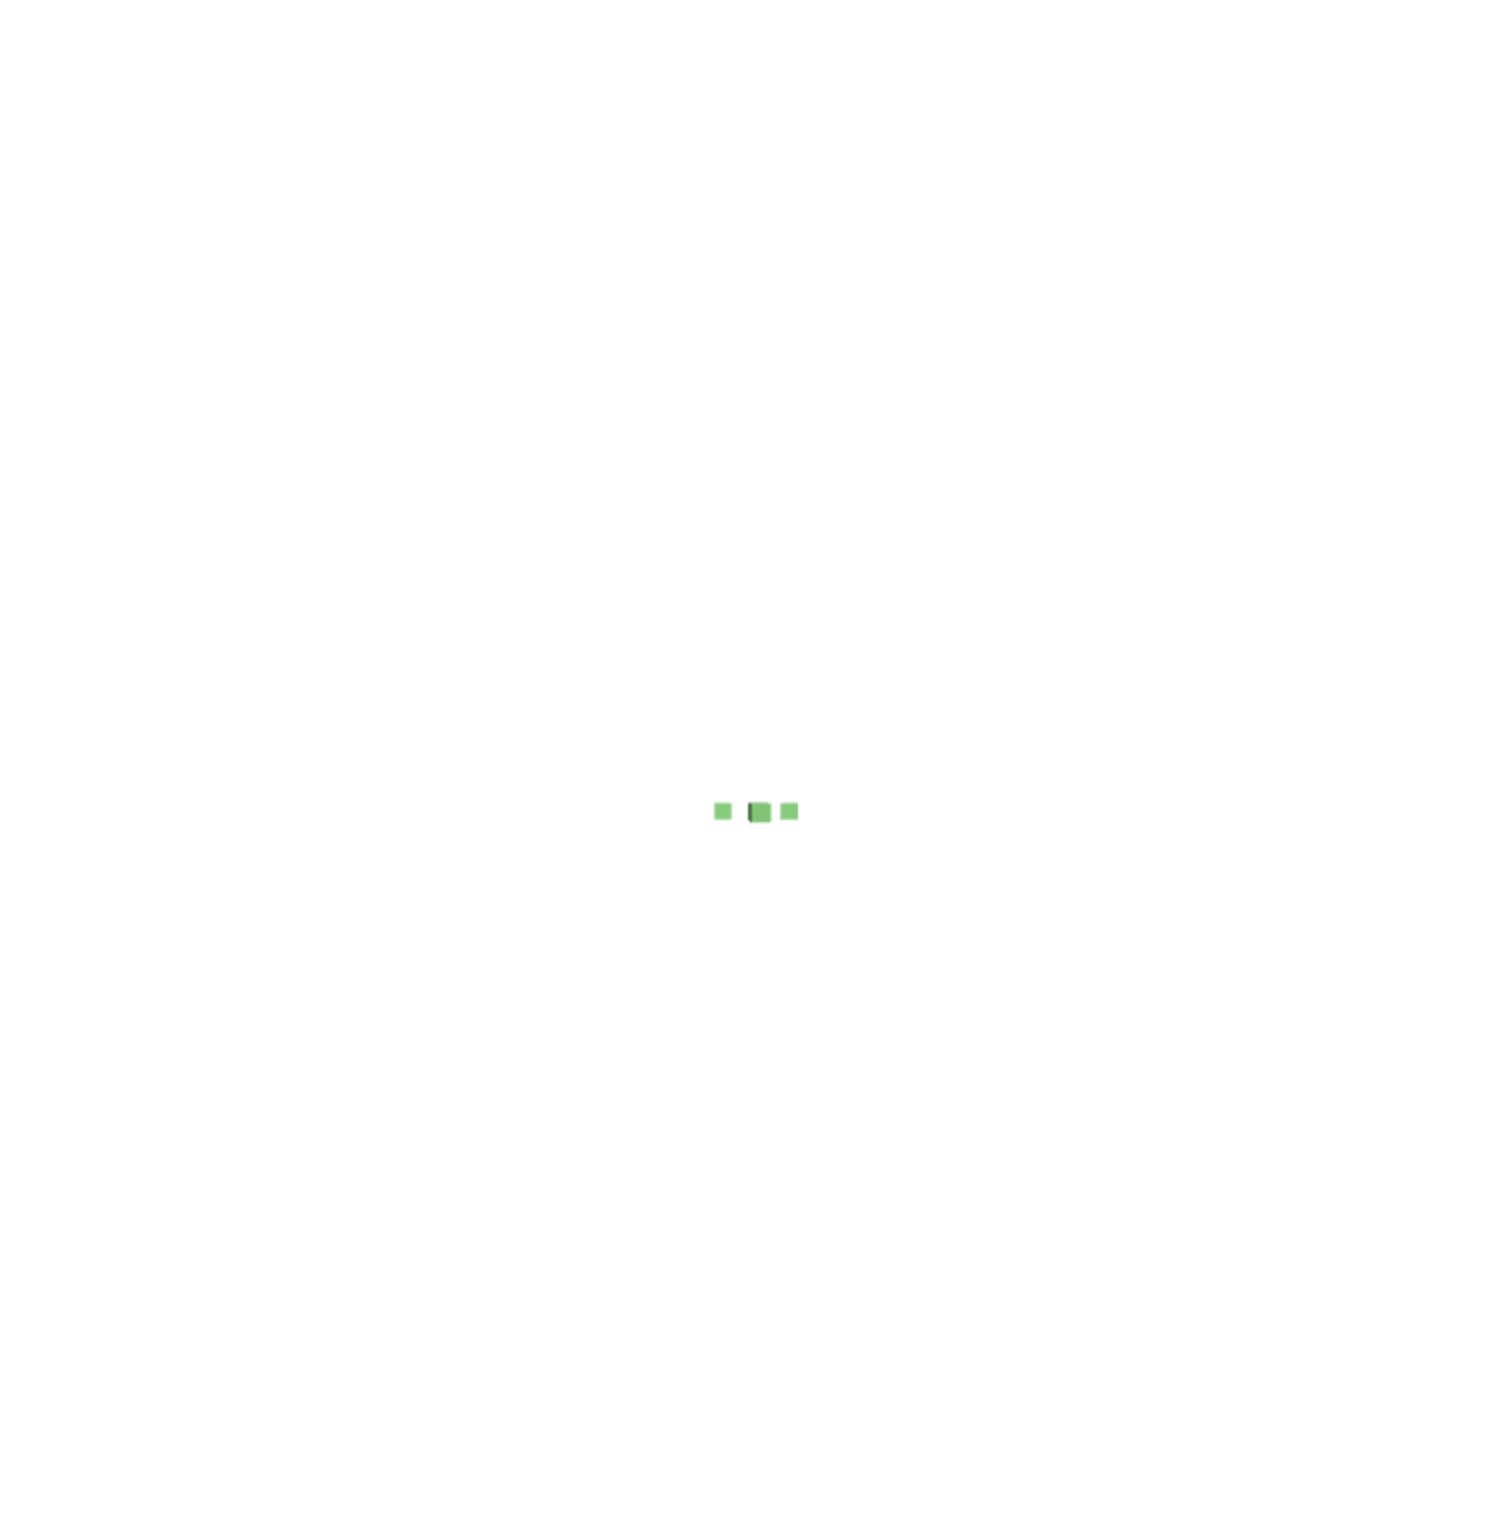
\includegraphics[width=\linewidth]{JetUML_V0S1.png}
        \caption{First commit seen from a top angle } 
        \label{fig:JetUML_V0S1_0}
    \end{subfigure}
    \hspace*{\fill}
    \begin{subfigure}{0.42\textwidth}
        
\includegraphics[width=\linewidth]{JetUML_V0S1_1.png}
        \caption{First commit seen from a mid angle} 
        \label{fig:JetUML_V0S1_1}
    \end{subfigure}
    \caption{First commit of JetUML made on Wed, 07 Jan 2015, 18:59. Three entities have been added; they are depicted with the green color. The entity in the middle represents the license file, taller because its size is bigger than other files.} 
    \label{fig:JetUML_V0S1}
\end{figure}

Here we present some results that we found looking at the graphical evolution of JetUML. 
To keep this section short, we report only a subset of the most active commits below. 
\bigbreak
The history of the repository starts on January 7, 2015, when Martin Robillard made the first commit. 
This commit added three files: README, a license, and a gitingore. 
Figure \ref{fig:JetUML_V0S1} represents it with three entities. All of them have the same shape because we did not adopt different shapes in the specification but the height is different. The license file is taller than other entities because of its bigger size. 
\bigbreak
Fifteen minutes later, he pushed the initial codebase of a project named Violet, composed of 83 files and an updated version of the gitignore file. This commit is represented in figure \ref{fig:JetUML_V0S2}, where 83 green entities represent added files, one yellow entity represents the updated gitignore files, and two gray entities, the README and the license files added before, that were not touched.
\bigbreak
Forty minutes later, he made the first big refactor of the system, whose goal was to move the position of some fields in each class. This refactoring involved 49 files, and as we can see from figure \ref{fig:JetUML_V0S3} they are marked in yellow. 
\bigbreak
Three days later, after a series of light development tasks had been continuously made, he moved some classes from the Violet folder to a new one named Violetta. As we can notice from figure \ref{fig:JetUML_V0S4} moved classes are represented with light blue. 
\bigbreak
Twenty-six commits later, on January 22, 2015, they moved classes from Violet and Violetta under the JetUML package. This commit, represented in figure \ref{fig:JetUML_V0S5}, was the first when JetUML was officially used; it denotes its birth. 
\bigbreak
After this first implementation, the system gradually grew, doubling its size in less than two years. 
During this time interval, they have been made only small commits to solve open issues. There were some exceptions, displayed in figure \ref{fig:JetUML_V0S6} and \ref{fig:JetUML_V0S7} where lots of files were modified because they had to update classes copyright lines. 
\bigbreak
In November 2017, they removed "stg" from the path of all the Java classes part of the system. This commit is depicted in figure \ref{fig:JetUML_V0S8}, where we can observe 162 light blue entities. They represent classes moved from the "../ca/mcgill/cs/stg/jetuml/..." path to the 
"../ca/mcgill/cs/jetuml/..." path. Moreover, this commit also had 15 modified fields, and one added. 
\bigbreak
One last huge refactor was done in July 2020, two years later, again to change the copyright on every class. It is represented in figure \ref{fig:JetUML_V0S9}. In this figure, we can notice that there are many blank spots in the middle. This means that entities added in the early stages of the project have been removed and are no longer part of the system. At that time, the system had 316 entities, and 241 were affected by this commit. 
\bigbreak
The last version of the system, created on Thu, 12 May 2022, counts 456 entities. 
\bigbreak
\textbf{Conclusion}
We manually inspected 2153 frames depicting the evolution of JetUML.
Thanks to the autoplay feature of SYN-Debugger, it was not an agonizing activity. \\
Occasionally JetUML needed to make huge commits involving the majority of files on their repository. Nonetheless, they were spotted easily, thanks to the adopted visualization settings. 
Most of the commits involved few entities; this means that features were implemented gradually, maybe following an incremental or spiral development approach. 
With this grouping strategy, it was hard to understand the regularity and the speed of the development process. This is normal when we traverse the history by commit rather than traverse it by time. 

\begin{figure}[t!]
    \begin{subfigure}{0.32\textwidth}
        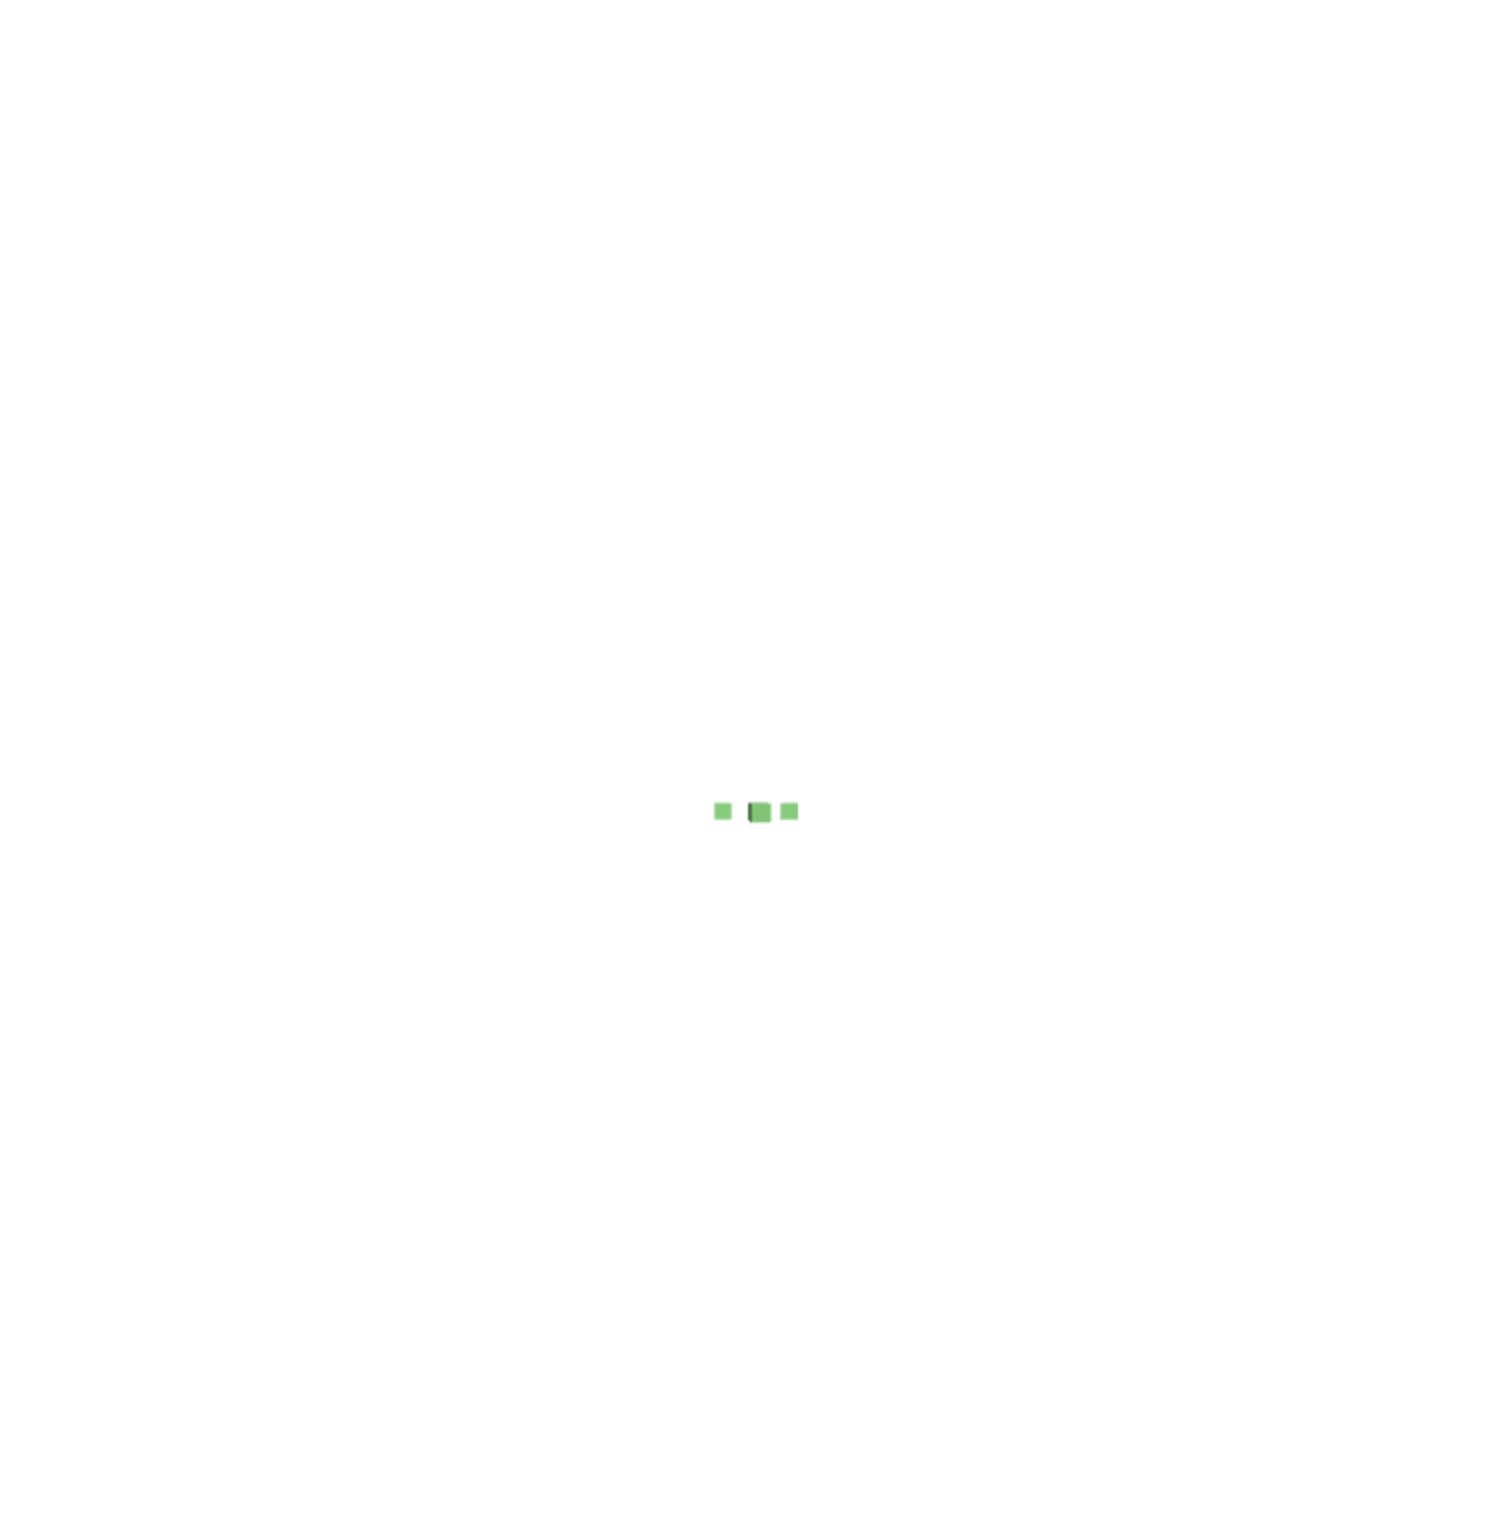
\includegraphics[width=\linewidth]{JetUML_V0S1.png}
        \caption{07 Jan 2015, 18:59 \linebreak Initial commit} \label{fig:JetUML_V0S1_3}
    \end{subfigure}
    \hspace*{\fill}
    \begin{subfigure}{0.32\textwidth}
        
\includegraphics[width=\linewidth]{JetUML_V0S2.png}
        \caption{07 Jan 2015, 19:14 \linebreak  Initial Revision} \label{fig:JetUML_V0S2}
    \end{subfigure}
    \hspace*{\fill}
    \begin{subfigure}{0.32\textwidth}
        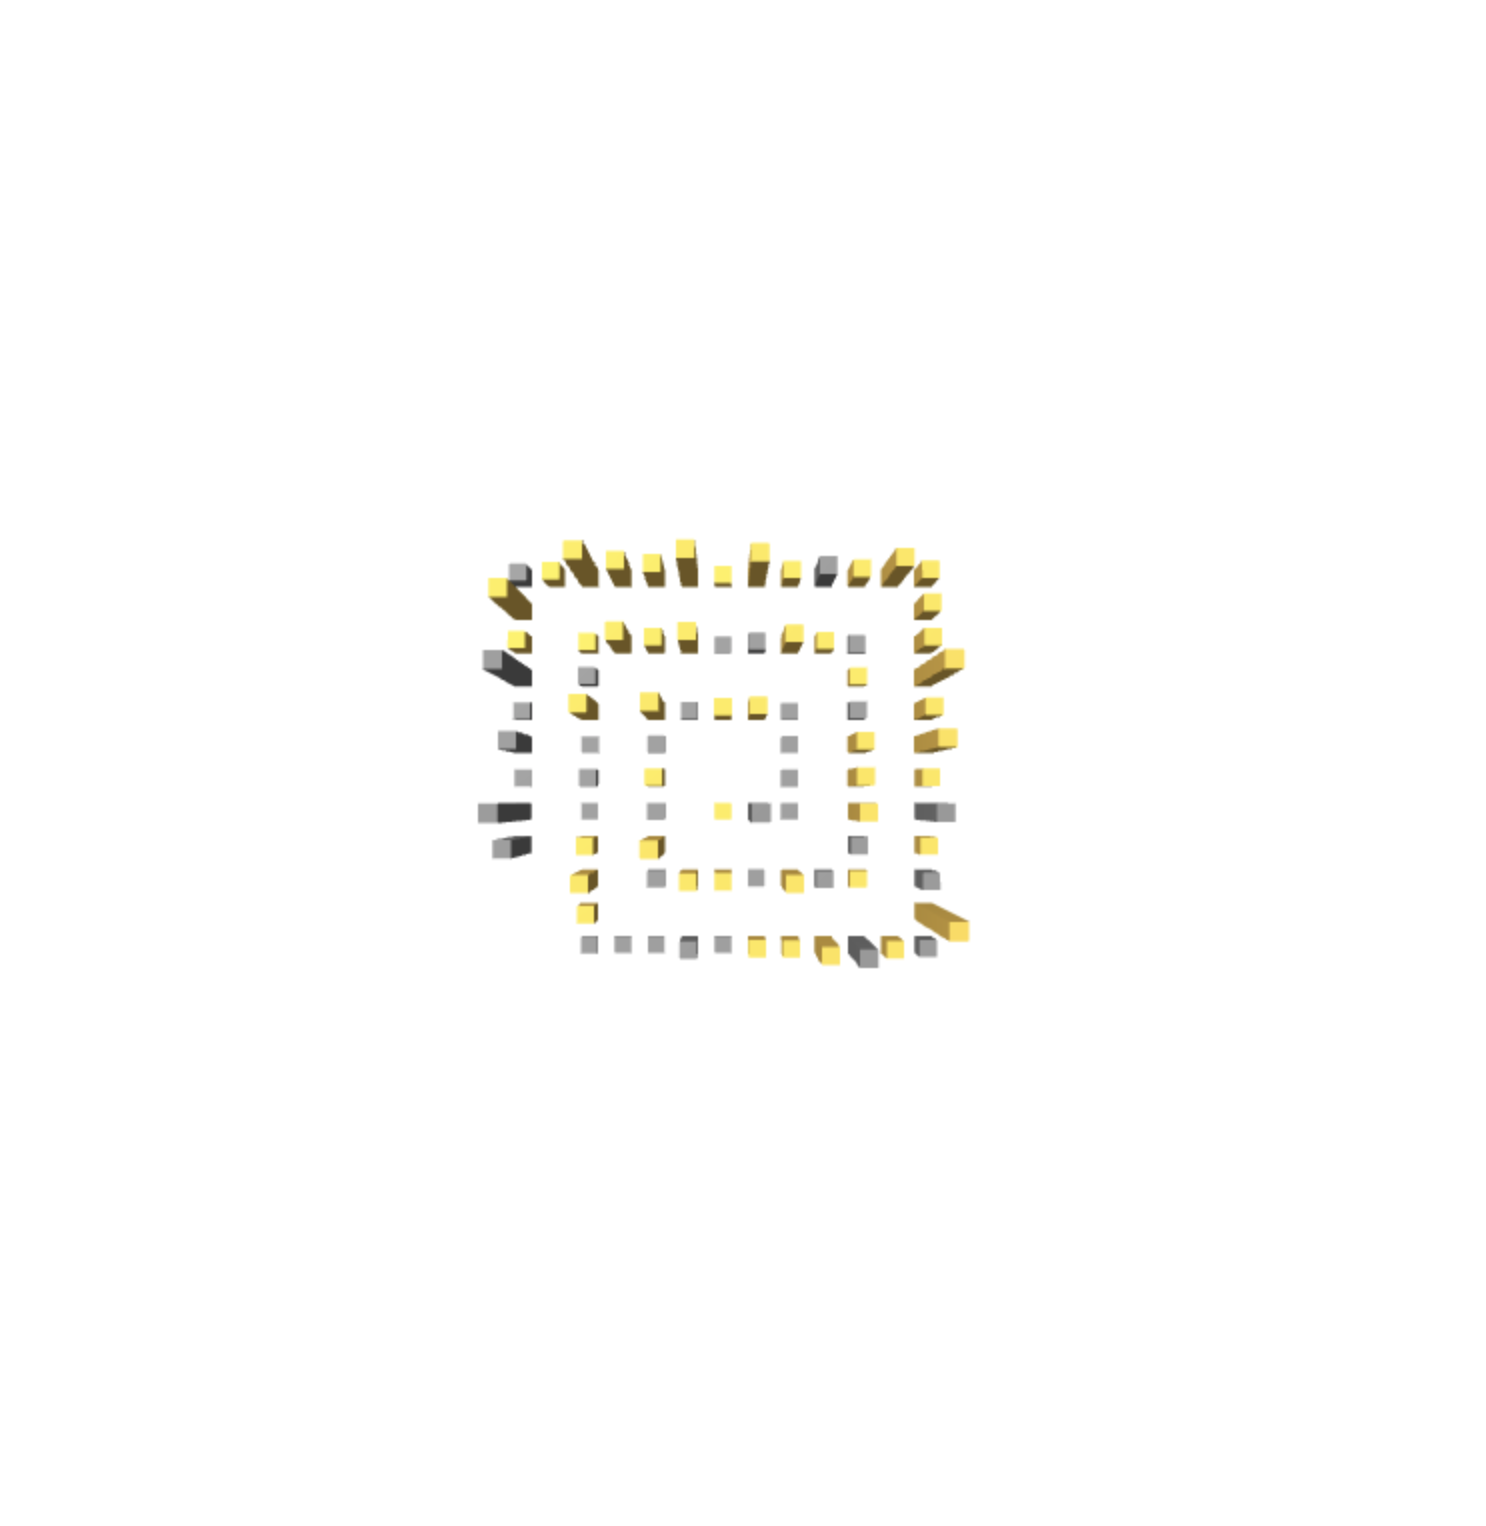
\includegraphics[width=\linewidth]{JetUML_V0S3.png}
        \caption{07 Jan 2015, 19:57 \linebreak  \#1 Move all fields} \label{fig:JetUML_V0S3}
    \end{subfigure}
    \hspace*{\fill}
    \medskip
    \begin{subfigure}{0.32\textwidth}
        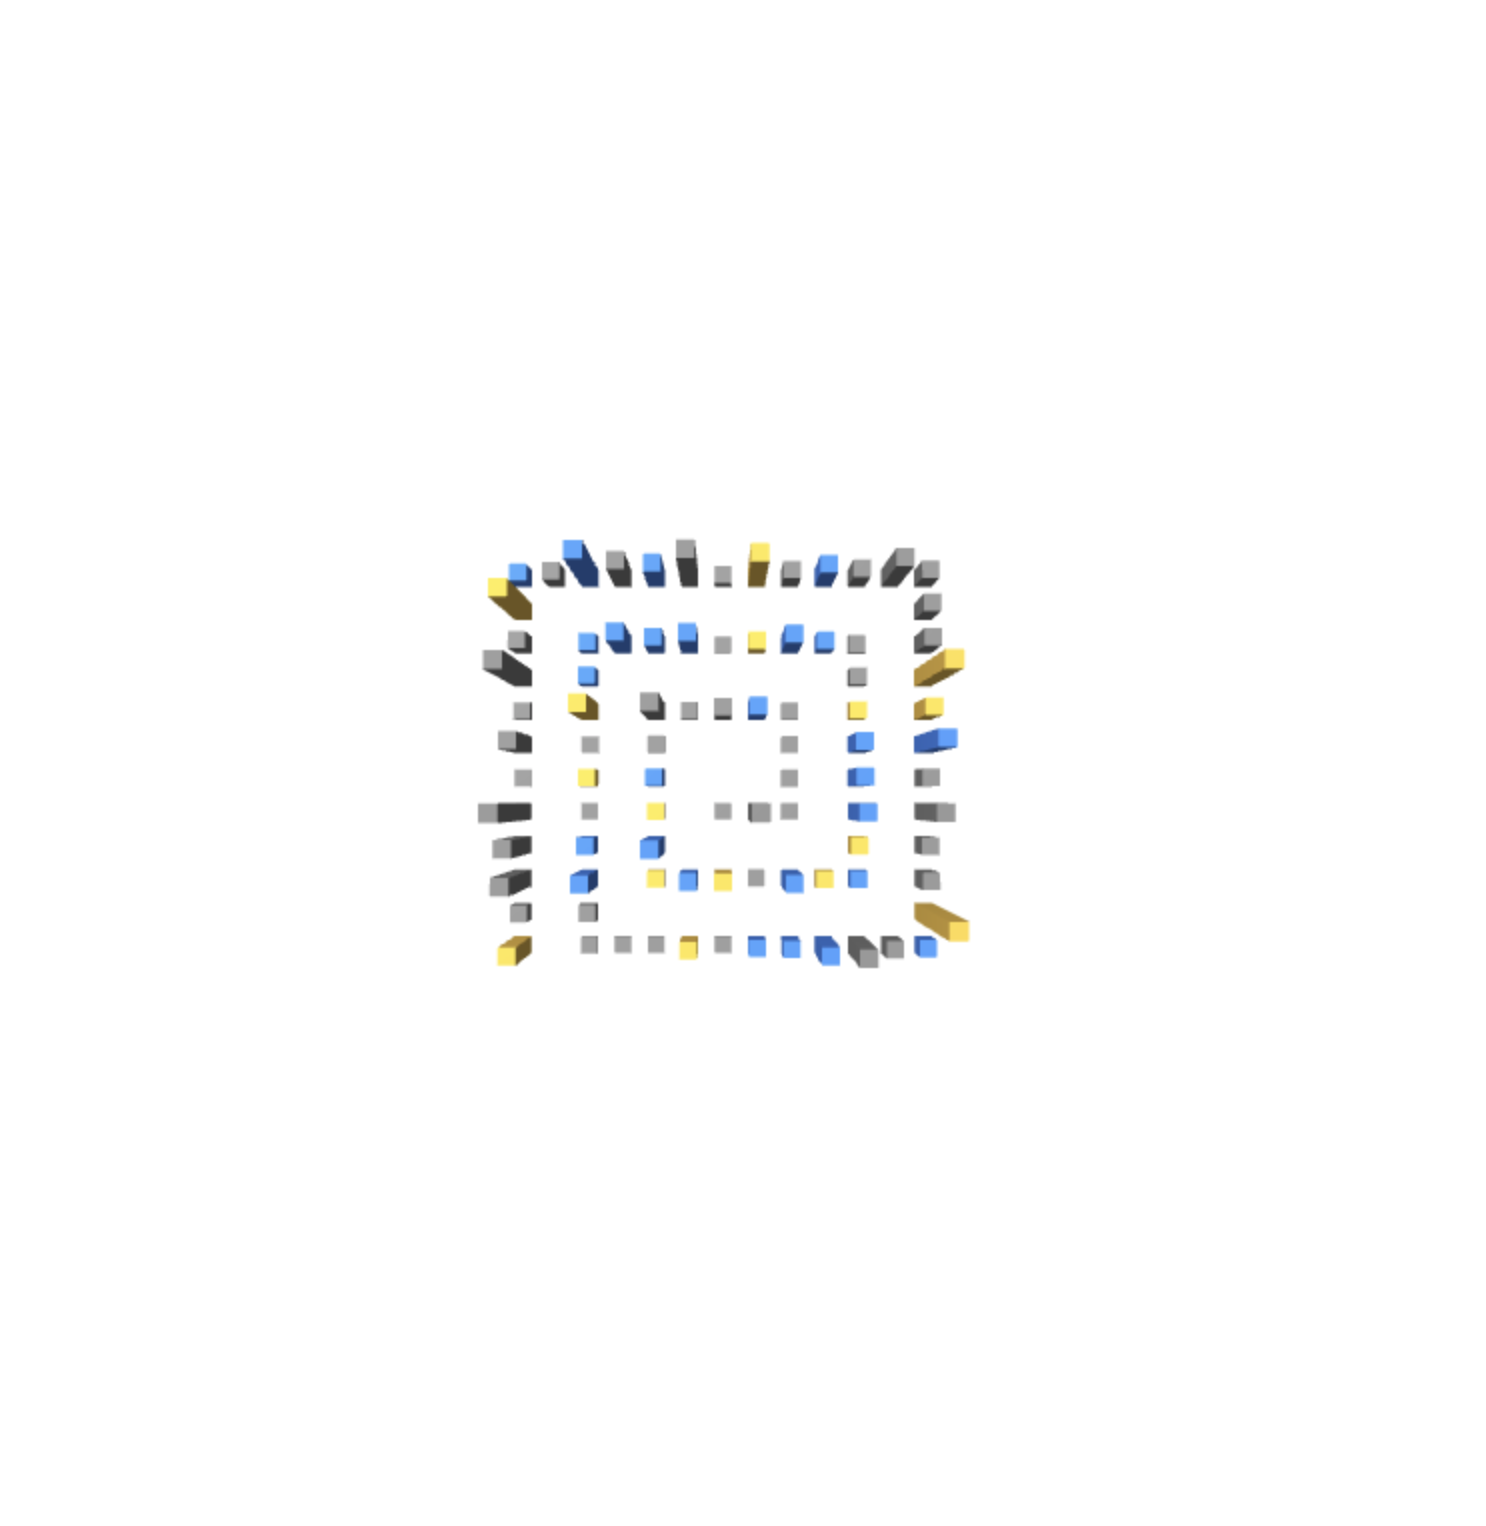
\includegraphics[width=\linewidth]{JetUML_V0S4.png}
        \caption{10 Jan 2015 \linebreak  \#8 Moved to a dedicated ...} 
        \label{fig:JetUML_V0S4}
    \end{subfigure}
    \hspace*{\fill}
    \begin{subfigure}{0.32\textwidth}
        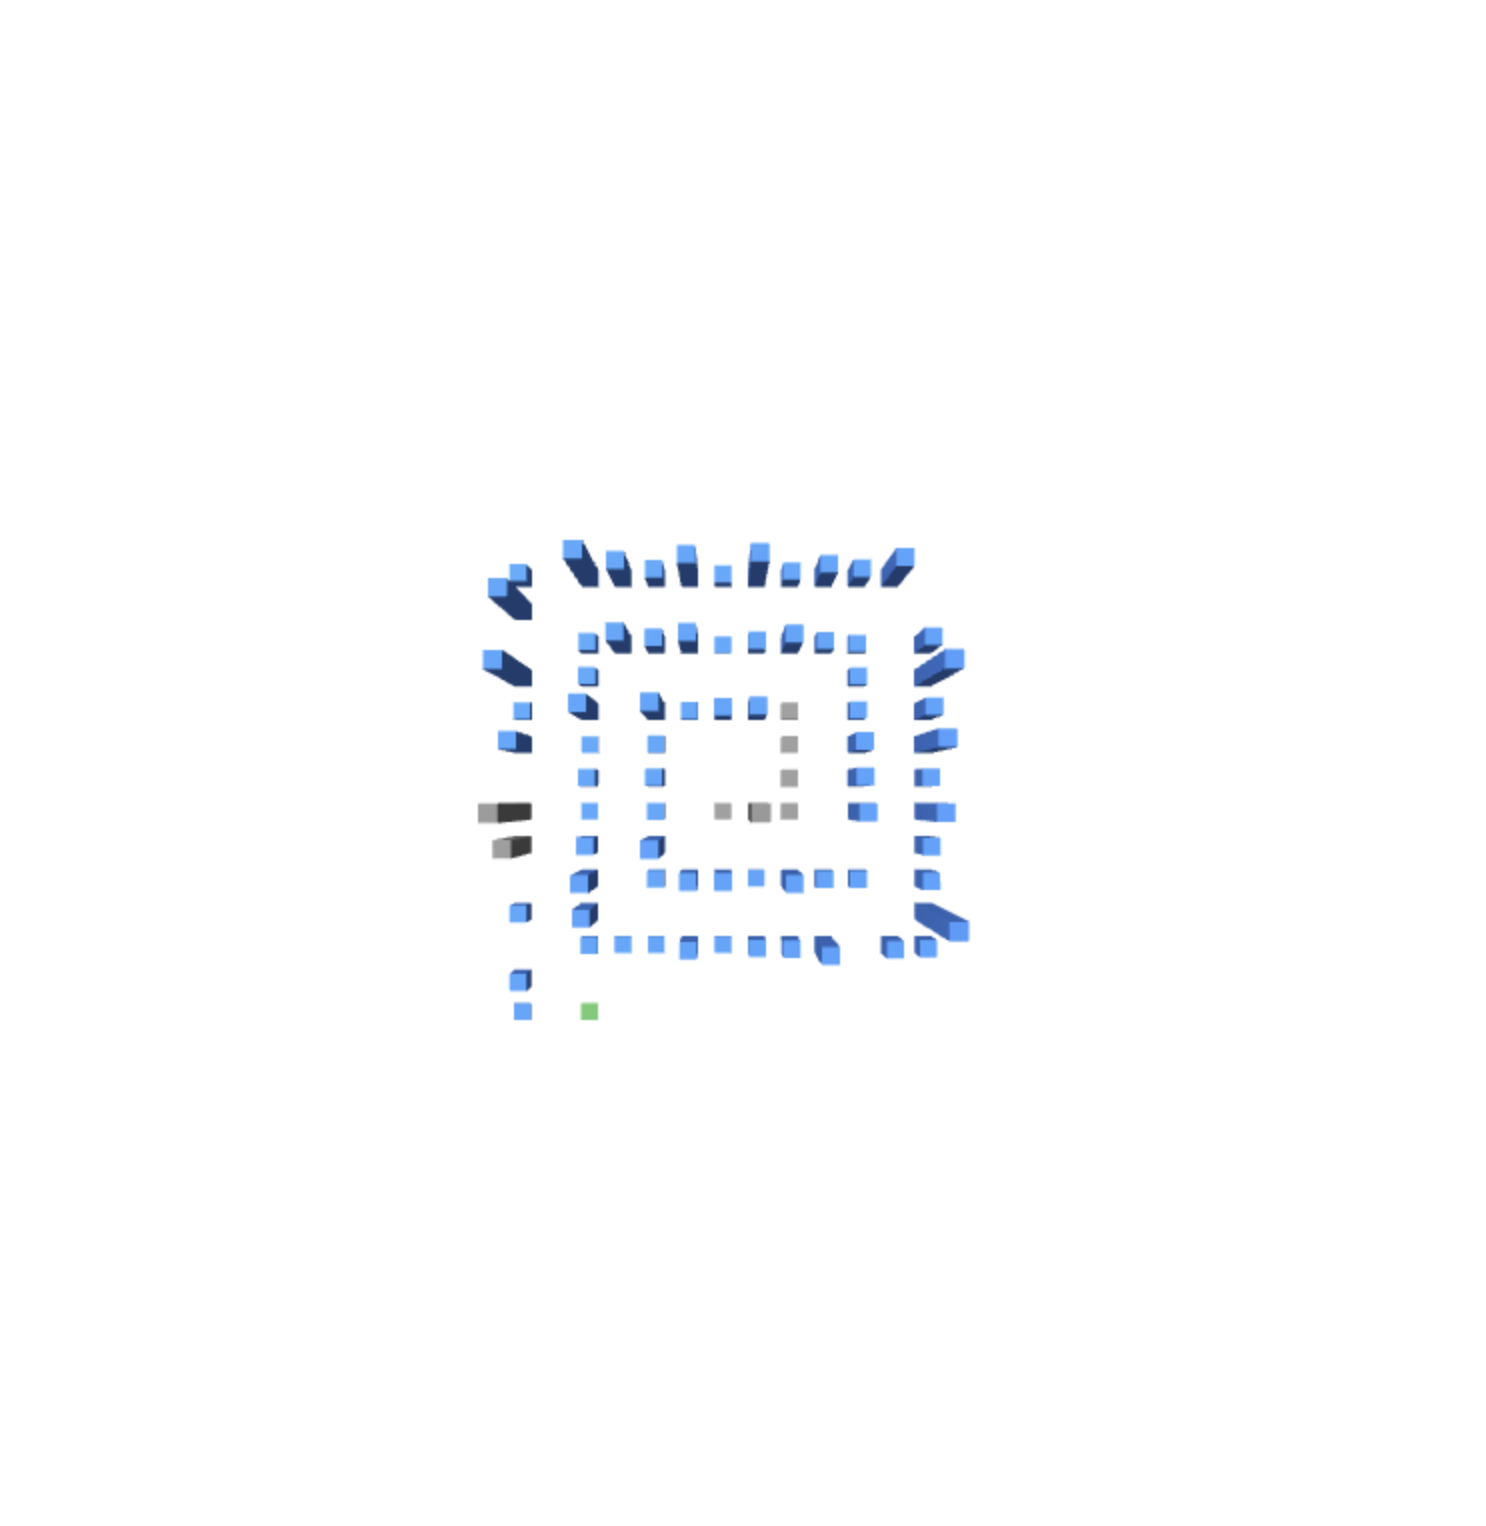
\includegraphics[width=\linewidth]{JetUML_V0S5.png}
        \caption{22 Jan 2015 \linebreak  \#27 Renamed the packages} 
        \label{fig:JetUML_V0S5}
    \end{subfigure}
    \hspace*{\fill}
    \begin{subfigure}{0.32\textwidth}
        
\includegraphics[width=\linewidth]{JetUML_V0S6.png}
        \caption{16 Oct 2015 \linebreak  \#3 New copyright block on ...} 
        \label{fig:JetUML_V0S6}
    \end{subfigure}
    \hspace*{\fill}
    \medskip
    \begin{subfigure}{0.32\textwidth}
        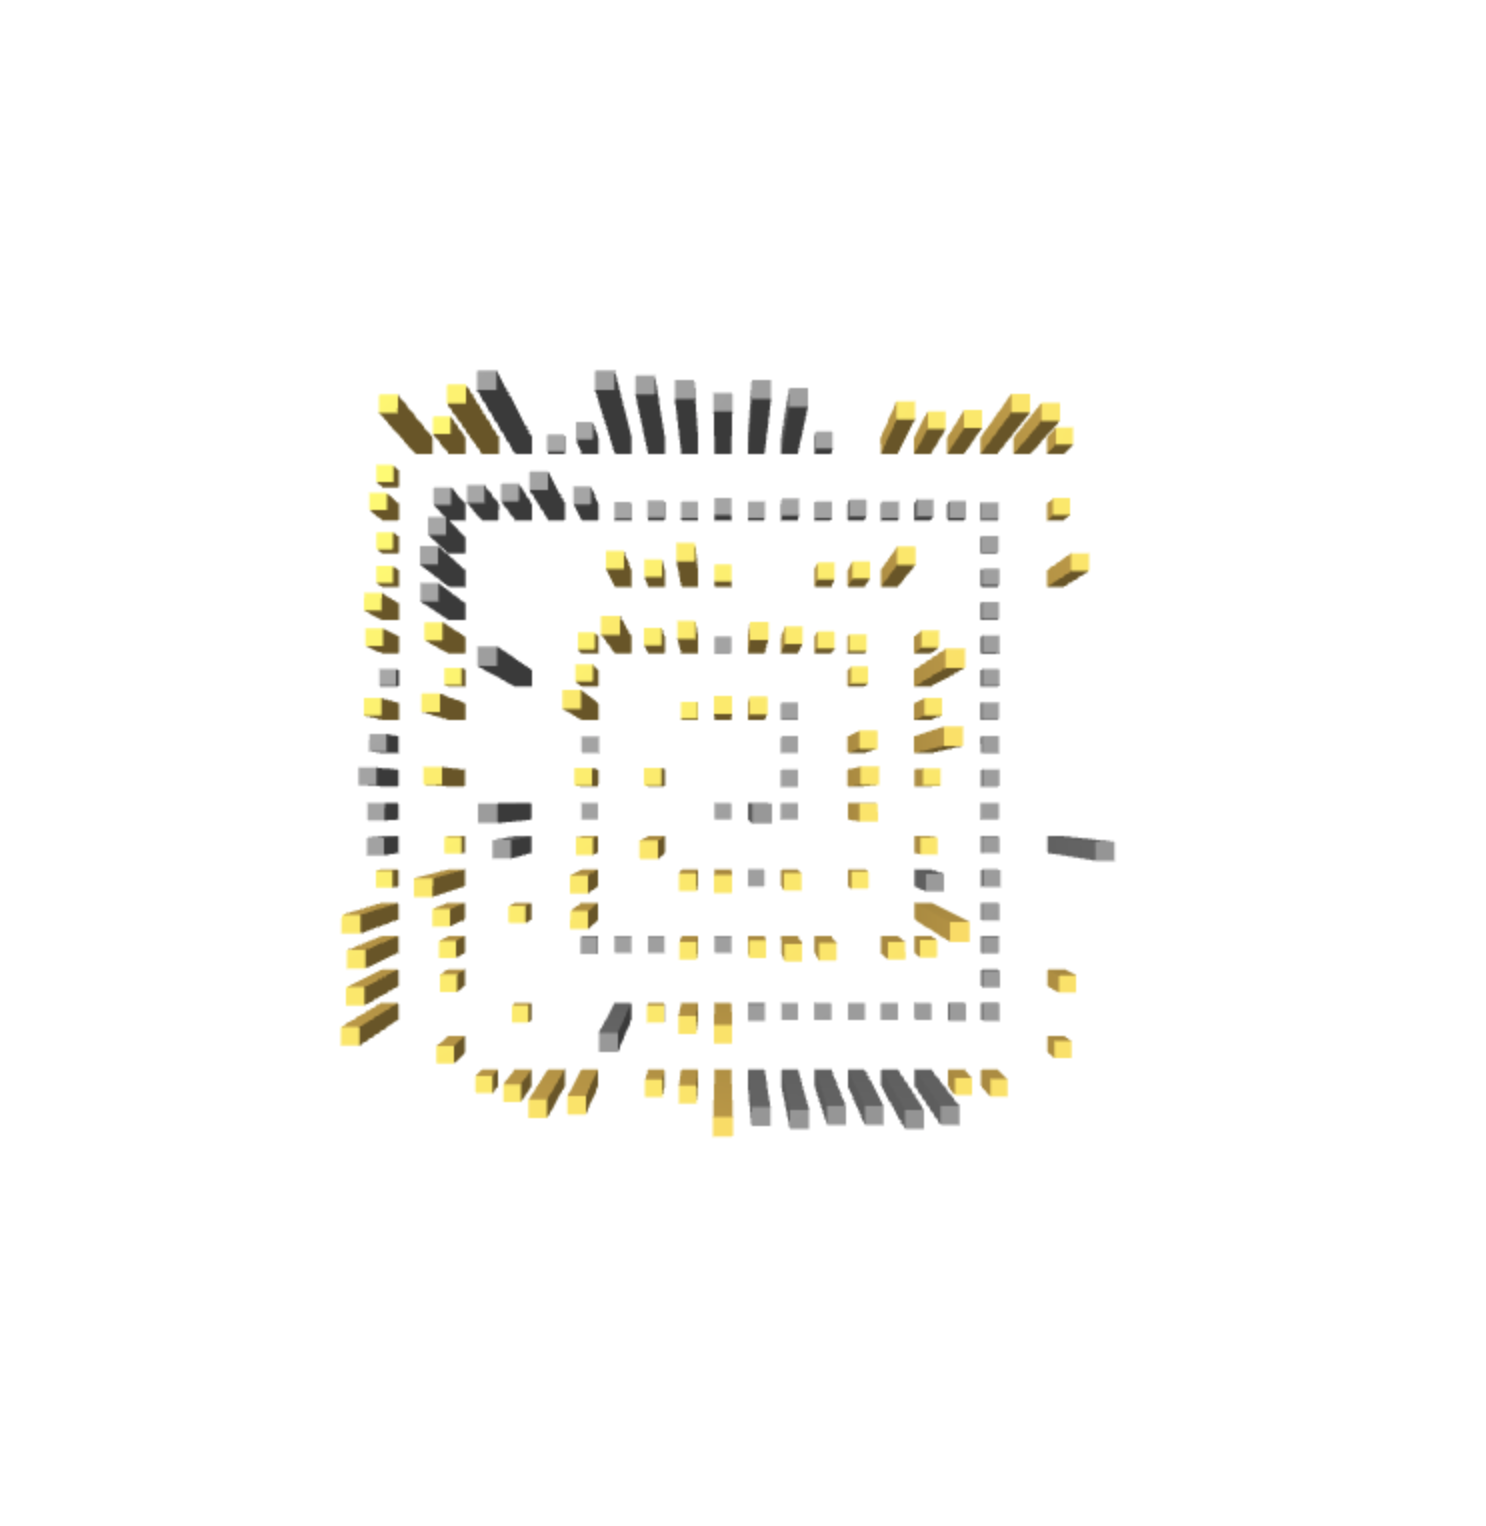
\includegraphics[width=\linewidth]{JetUML_V0S7.png}
        \caption{17 Jan 2016 \linebreak  \#146 Updated the copyright ...}
         \label{fig:JetUML_V0S7}
    \end{subfigure}
    \hspace*{\fill}
    \begin{subfigure}{0.32\textwidth}
        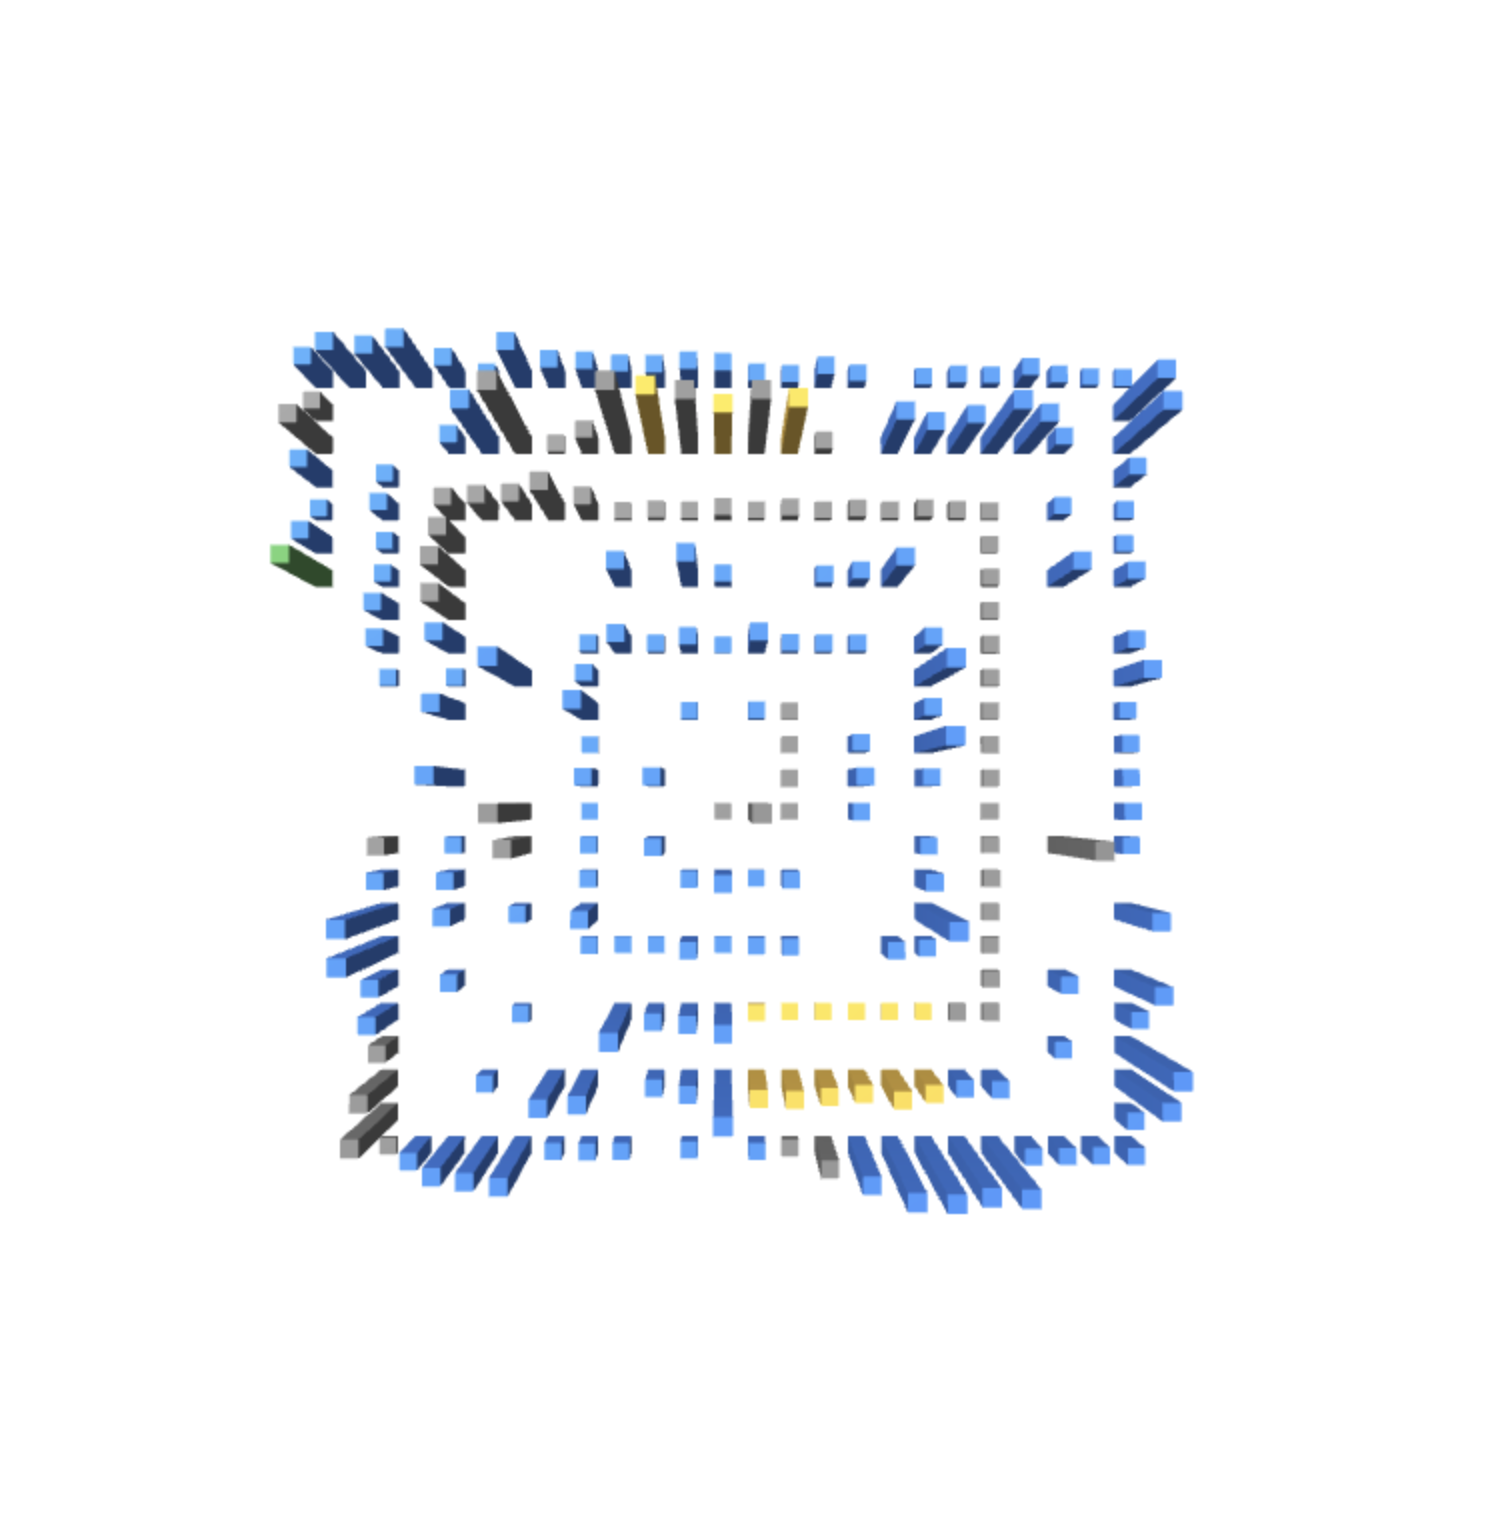
\includegraphics[width=\linewidth]{JetUML_V0S8.png}
        \caption{26 Nov 2017 \linebreak  \#212 Remove stg from name} 
    \label{fig:JetUML_V0S8}
    \end{subfigure}
    \hspace*{\fill}
    \begin{subfigure}{0.32\textwidth}
        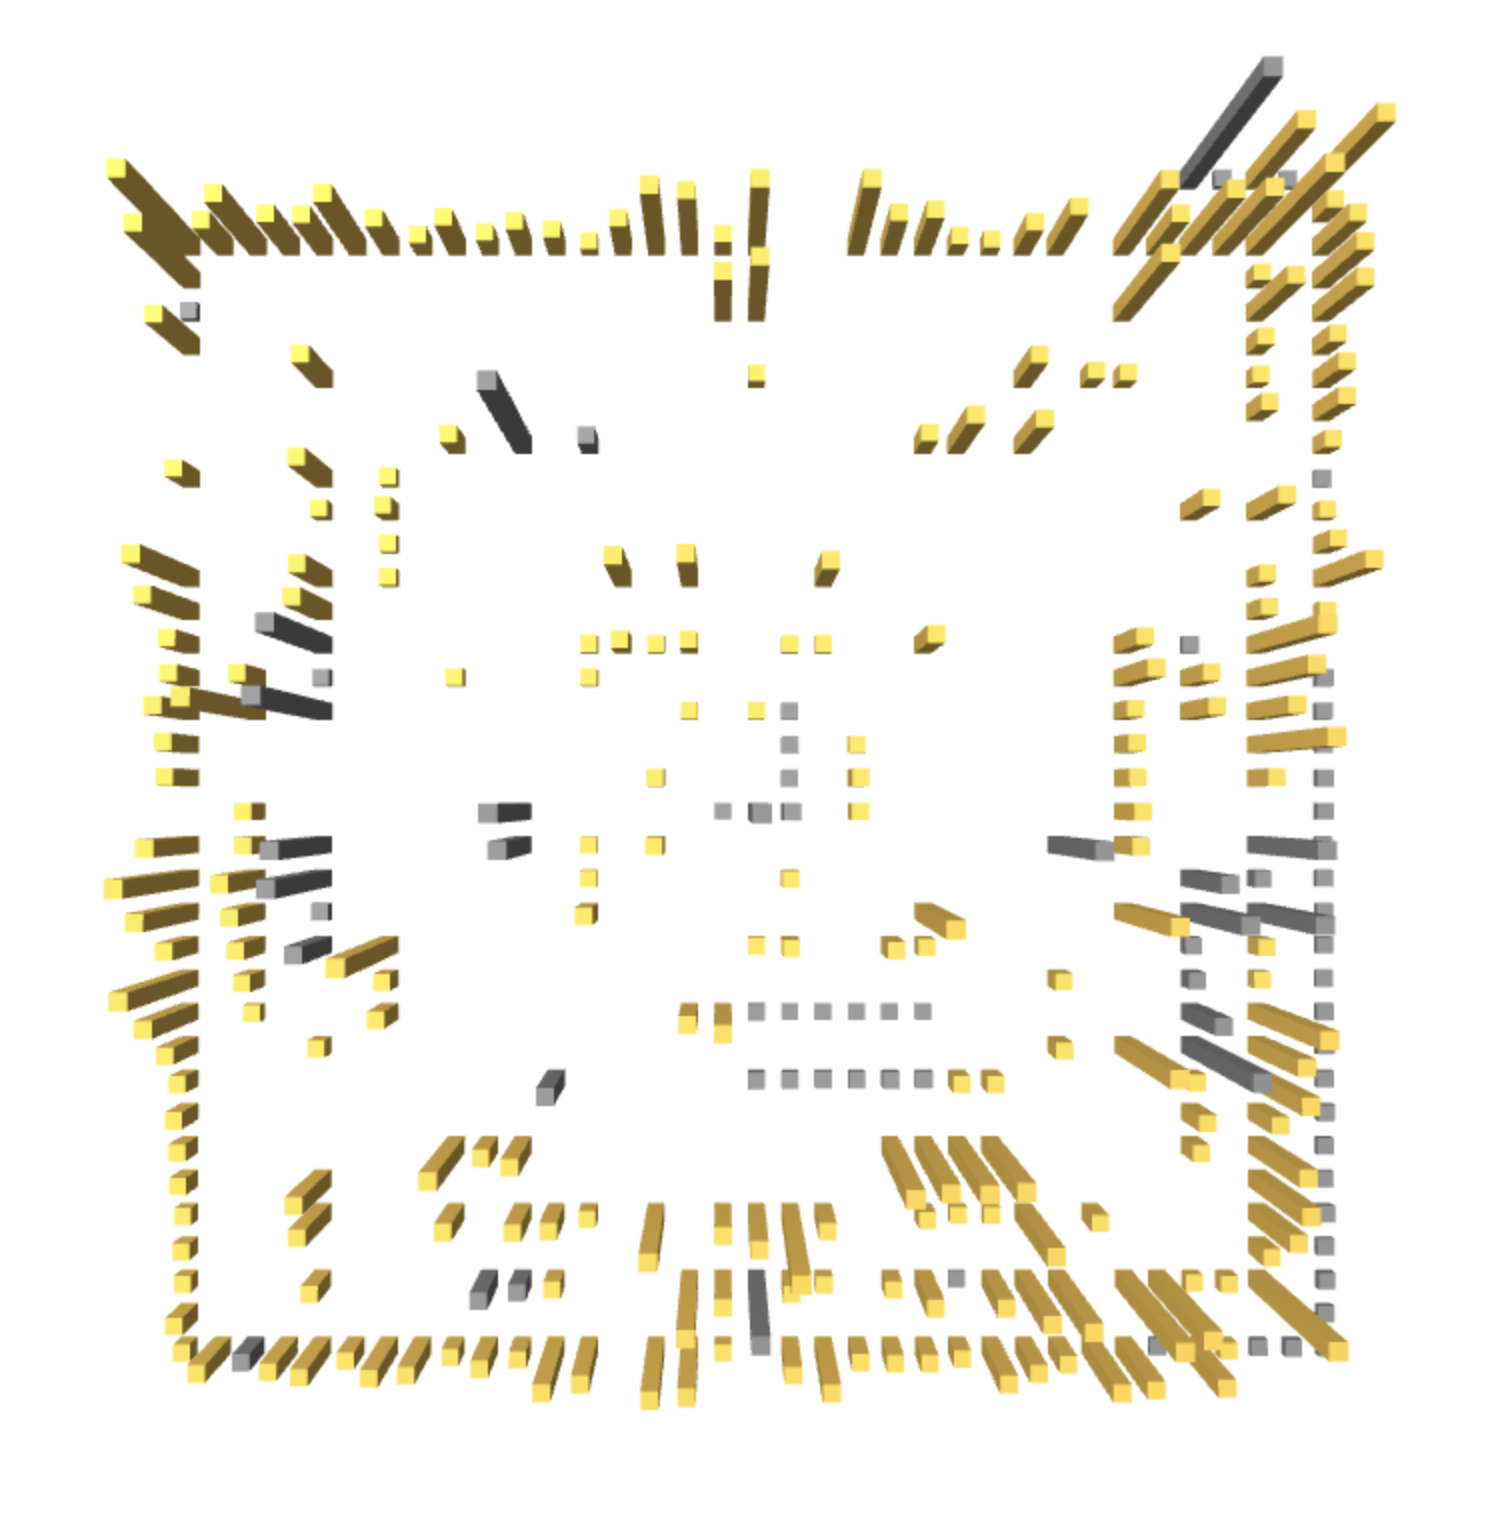
\includegraphics[width=\linewidth]{JetUML_V0S9.png}
        \caption{22 Jul 2020 \linebreak  \#374 Fix copyrights} \label{fig:JetUML_V0S9}
    \end{subfigure}
    \hspace*{\fill}
    \medskip
    \caption{
        Subset of the biggest commits in JetUML. Figure \ref{fig:JetUML_V0S1_3} represent the first commit. In Figure \ref{fig:JetUML_V0S2} they pushed the code of Violetta. Figure \ref{fig:JetUML_V0S3} depicts their first refactoring. In Figure \ref{fig:JetUML_V0S4} they moved some classes from Violet to Violetta. In Figure  \ref{fig:JetUML_V0S5} they moved most of them under JetUML. In Figure \ref{fig:JetUML_V0S6}, \ref{fig:JetUML_V0S7} and \ref{fig:JetUML_V0S9} are depicted three refactoring activities to fix copyrights. In Figure \ref{fig:JetUML_V0S8} most of the entities are painted with blue because they changed their path.} 
    \label{fig:JetUML_V0}
\end{figure}


\newpage
\subsubsection*{View 1}
\textbf{Goal of this visualization}
With this visualization, we want to see how all JetUML files evolved through time. 
JetUML does not seem to have a fixed release cycle.
Since its history spans eight years of activity, we initially chose a timestamp grouping strategy of one month. 
As a consequence, we have 89 AnimationFrames. 
In this first visualization, we do not care about the FileType of entities; we are interested in all of them. 
Grouping commits monthly; we applied the same strategy to the aging to see how many months had passed since an entity was modified. 
To summarize, the view specification of this visualization is the following:
\begin{itemize}
    \item \texttt{versionGroupingStrategy}: timestamp.
    \item \texttt{versionGroupingChunkSize}: 2'629'743 (1 month). 
    \item \texttt{colorPalette}: default, additions -> green, modifications -> orange, rename -> lightblue, moves -> blue.
    \item \texttt{agingGroupingStrategy}: timestamp.
    \item \texttt{agingStepSize}: 2'629'743 (1 month).
    \item \texttt{agingSteps}: 10 steps. 
    \item \texttt{mapperStrategy}: LinearBucketValueStrategy.
    \item \texttt{mapperStrategyOptions}: max height of 20.
    \item \texttt{mapperMetricName}: SIZE. 
    \item \texttt{showUnmappedEntities}: true.
    \item \texttt{fileTypeShape}: all boxes. 
    \item \texttt{fileTypeOpacity}: all 1. 
    \item \texttt{showDeletedEntities}: false.
\end{itemize}

\textbf{Results}
Figure \ref{fig:JetUML_V1} shows the first 6 month of evoluition of JetUML. 
We can infer many things by looking at these figures. In figure \ref{fig:JetUML_V1S1} 7 entities have been moved. 
Most of them are files with the extension \texttt{.properties} and perhaps they were involved in a refactoring activity since their path changed from
\texttt{src/ca/mcgill/cs/stg/jetuml/...} to \texttt{src/ca/mcgill/cs/stg/jetuml/diagrams/...}. 
At the end of their first month of activity, they had 135 files and made 127 commits. 
We can see many files are still green. This means that they were added but never touched after. 
An issue with this visualization is that we cannot distinguish Java files from others. 
These added files are images. Therefore it is not a surprise that once added; they are never modified in the future. 
In figure \ref{fig:JetUML_V1S2} where the second month is represented, we can see that some entities have a darker color. 
This means that during the second month, they were not touched. 
Comparing all the figures until figure \ref{fig:JetUML_V1S6} we can notice that many entities have the same behavior. 
They were added and updated in the first month of activity (this is the reason why they are yellow), and then they were never touched, becoming darker and darker each month. 

\begin{figure}[t!]
    \begin{subfigure}{0.48\textwidth}
    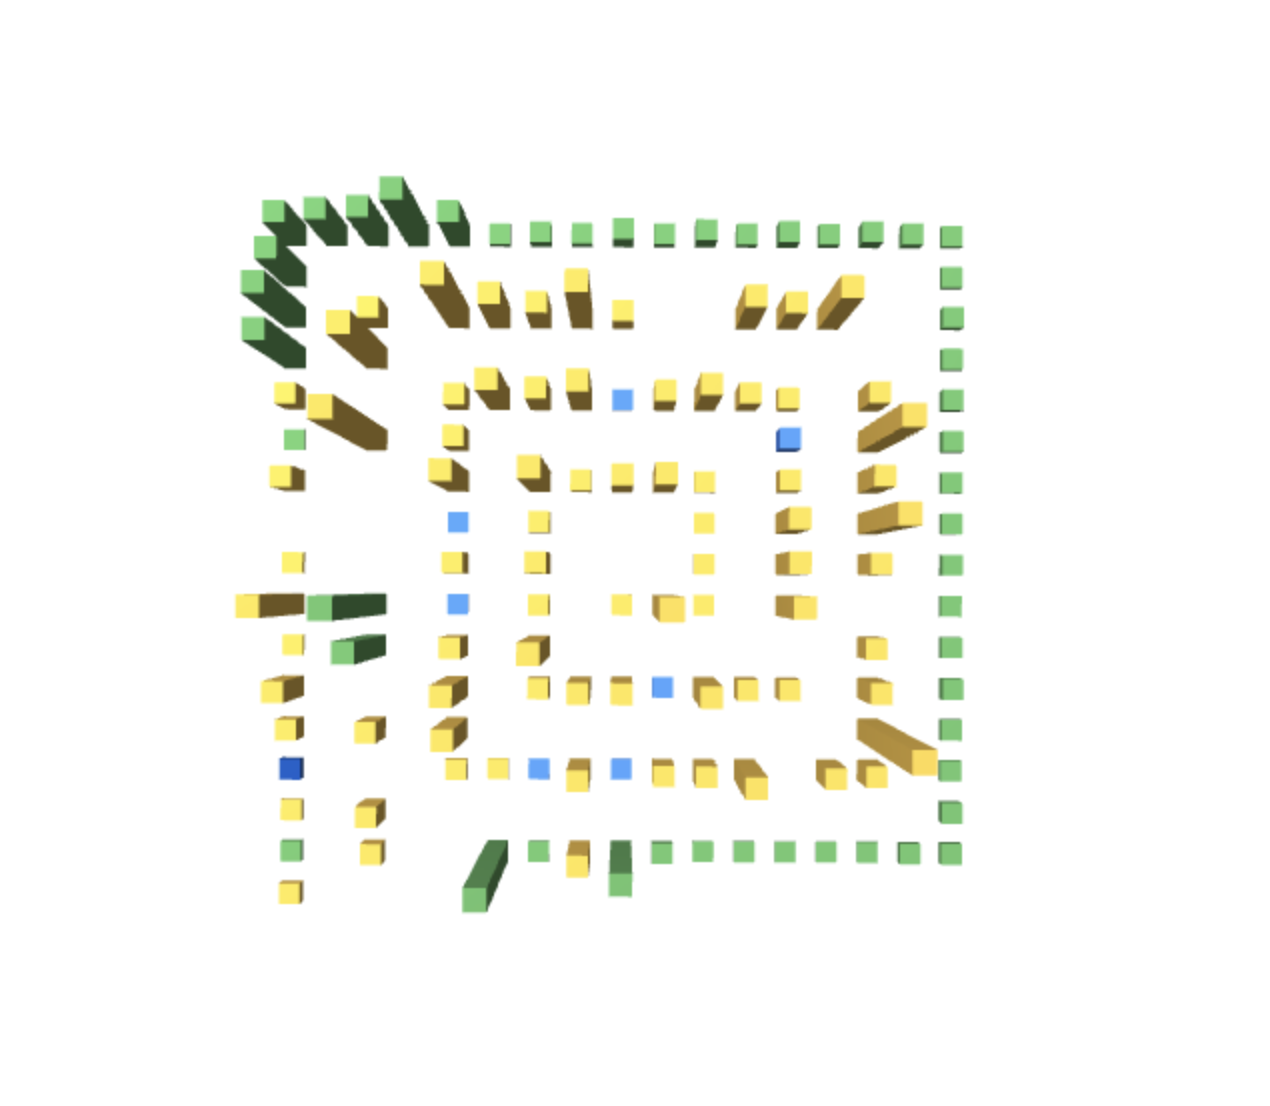
\includegraphics[width=\linewidth]{JetUML_V1S1.png}
    \caption{Month 1} \label{fig:JetUML_V1S1}
    \end{subfigure}\hspace*{\fill}
    \begin{subfigure}{0.48\textwidth}
        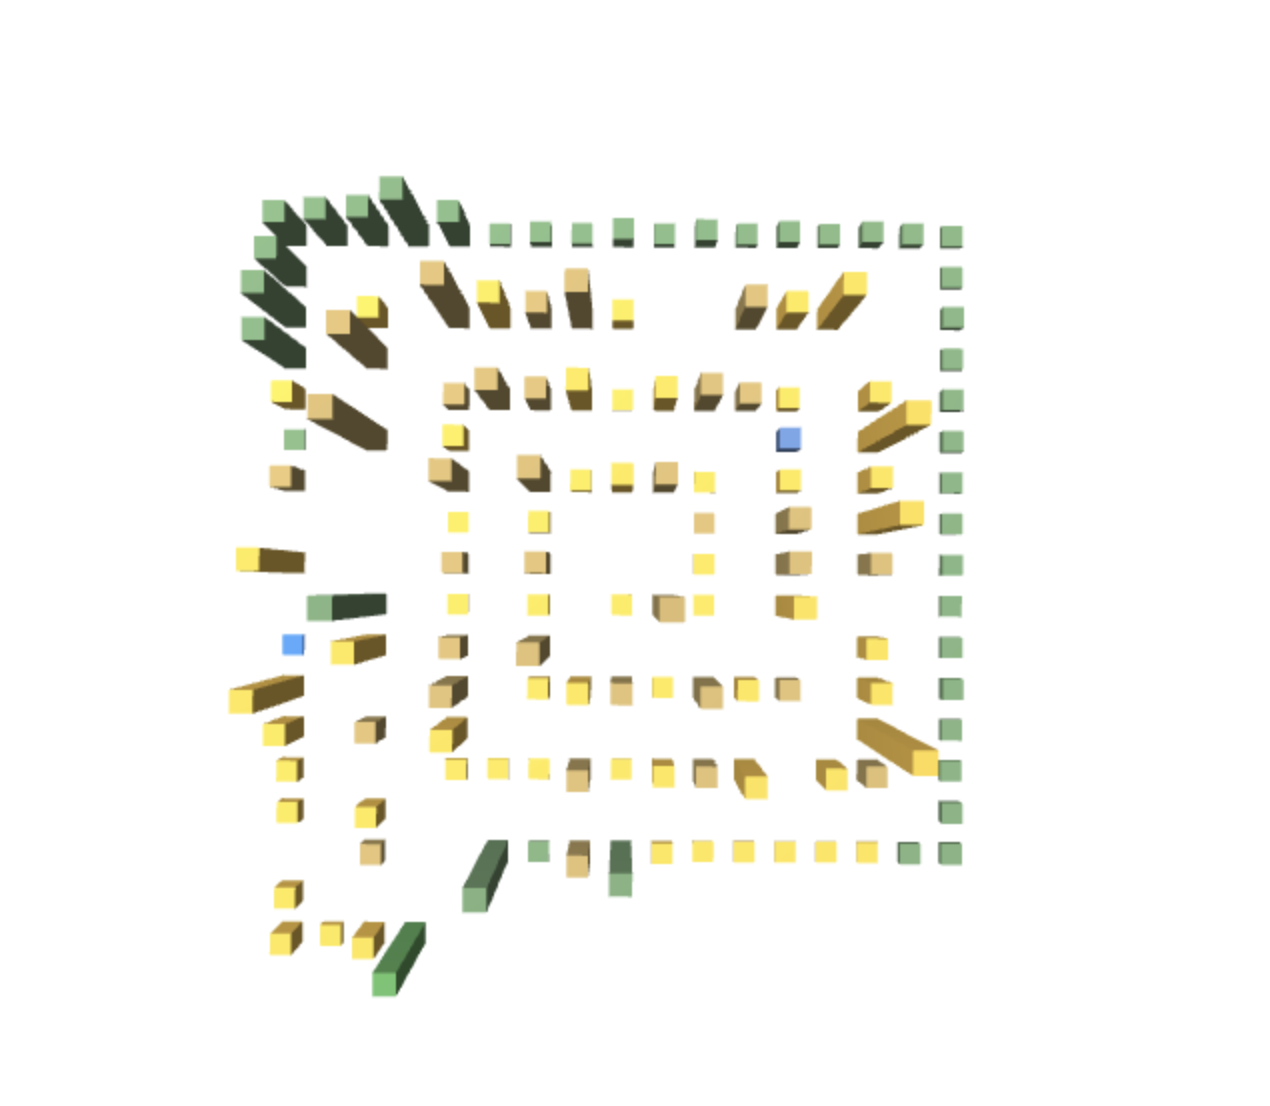
\includegraphics[width=\linewidth]{JetUML_V1S2.png}
        \caption{Month 2} \label{fig:JetUML_V1S2}
    \end{subfigure}
    
    \medskip
    \begin{subfigure}{0.48\textwidth}
        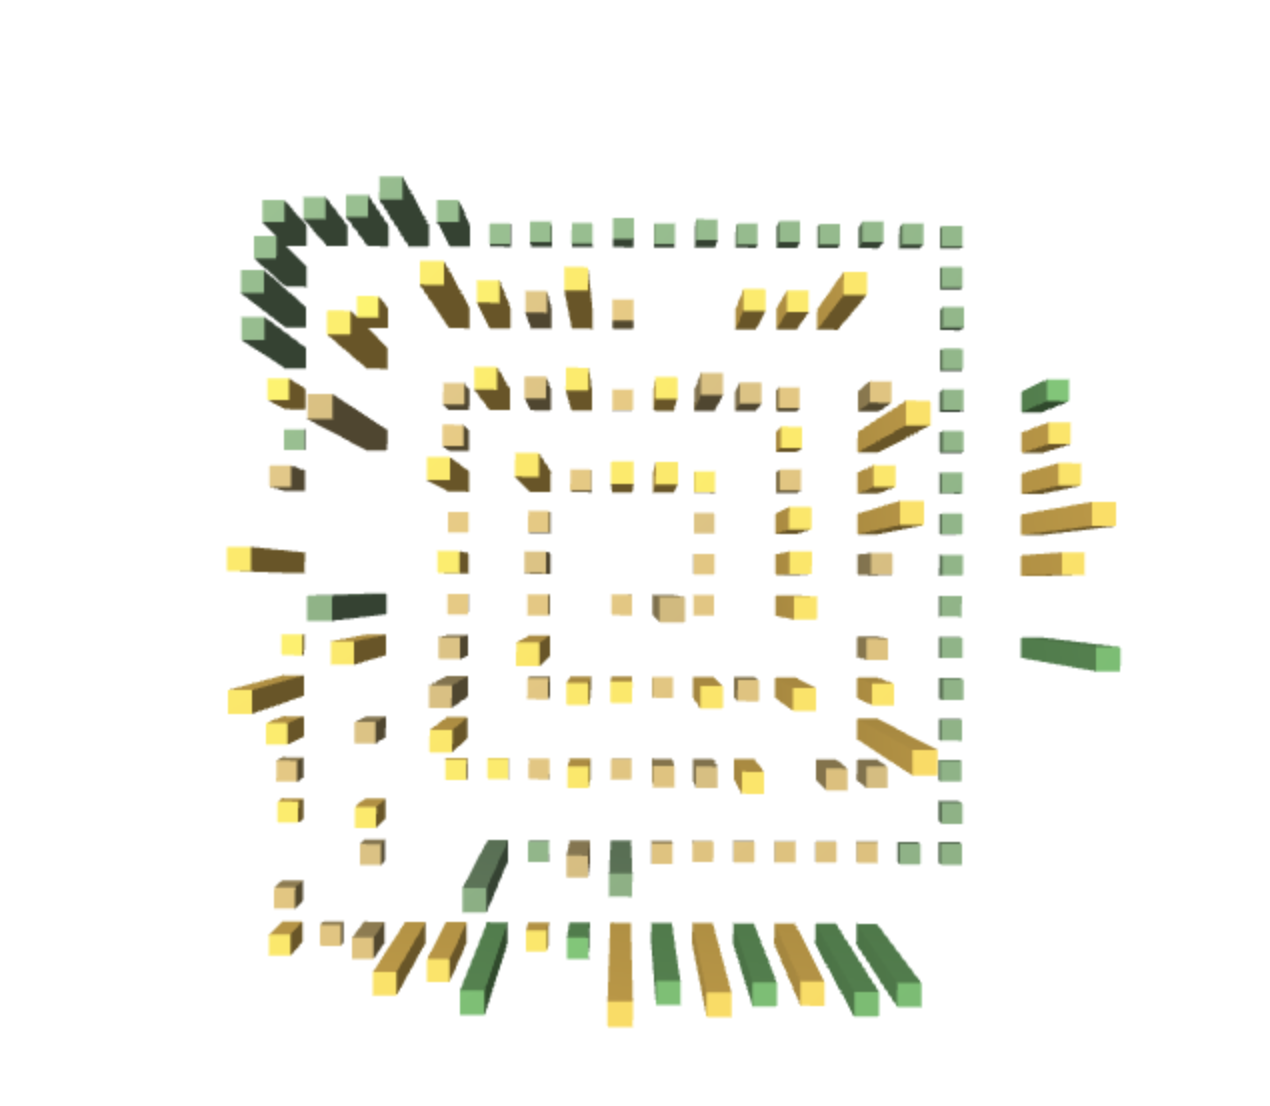
\includegraphics[width=\linewidth]{JetUML_V1S3.png}
        \caption{Month 3} \label{fig:JetUML_V1S3}
    \end{subfigure}\hspace*{\fill}
    \begin{subfigure}{0.48\textwidth}
    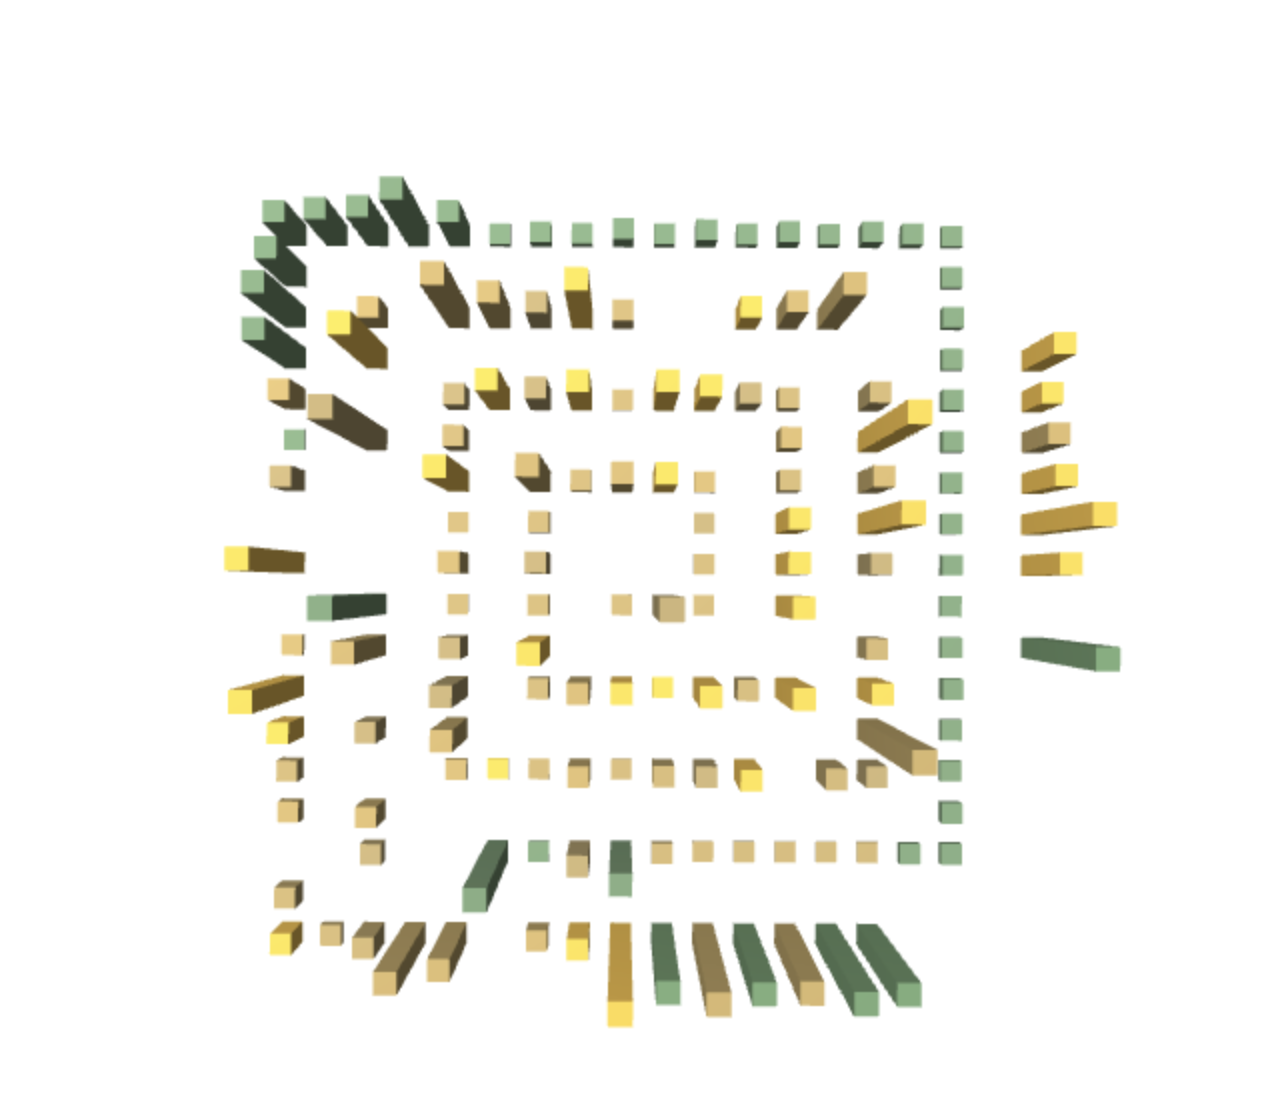
\includegraphics[width=\linewidth]{JetUML_V1S4.png}
    \caption{Month 4} \label{fig:JetUML_V1S4}
    \end{subfigure}
    
    \medskip
    \begin{subfigure}{0.48\textwidth}
        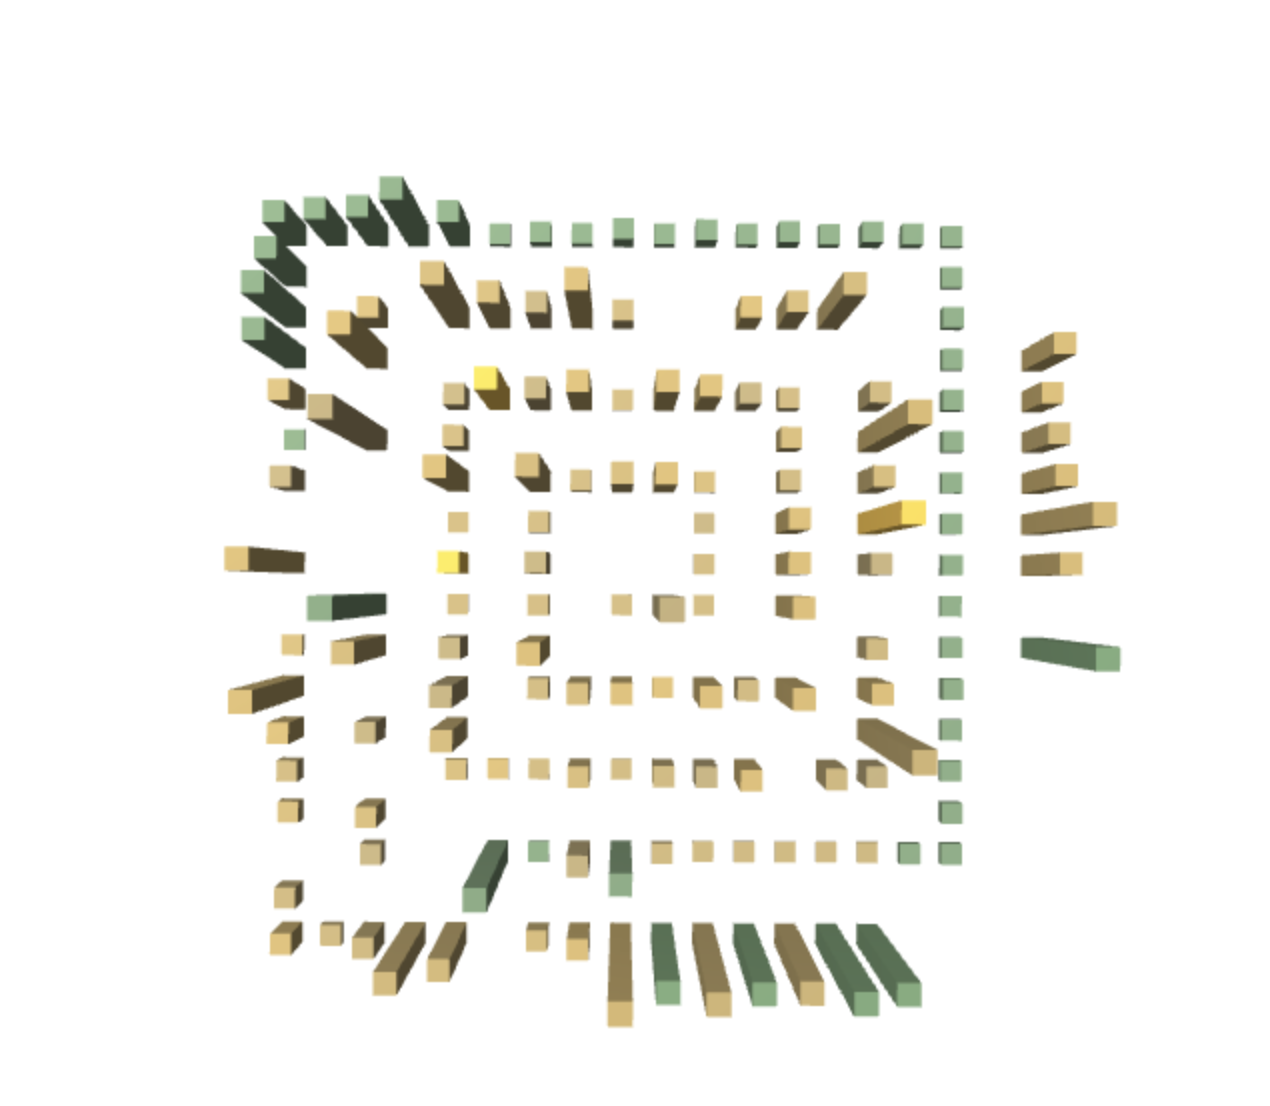
\includegraphics[width=\linewidth]{JetUML_V1S5.png}
        \caption{Month 5} \label{fig:JetUML_V1S5}
    \end{subfigure}\hspace*{\fill}
    \begin{subfigure}{0.48\textwidth}
        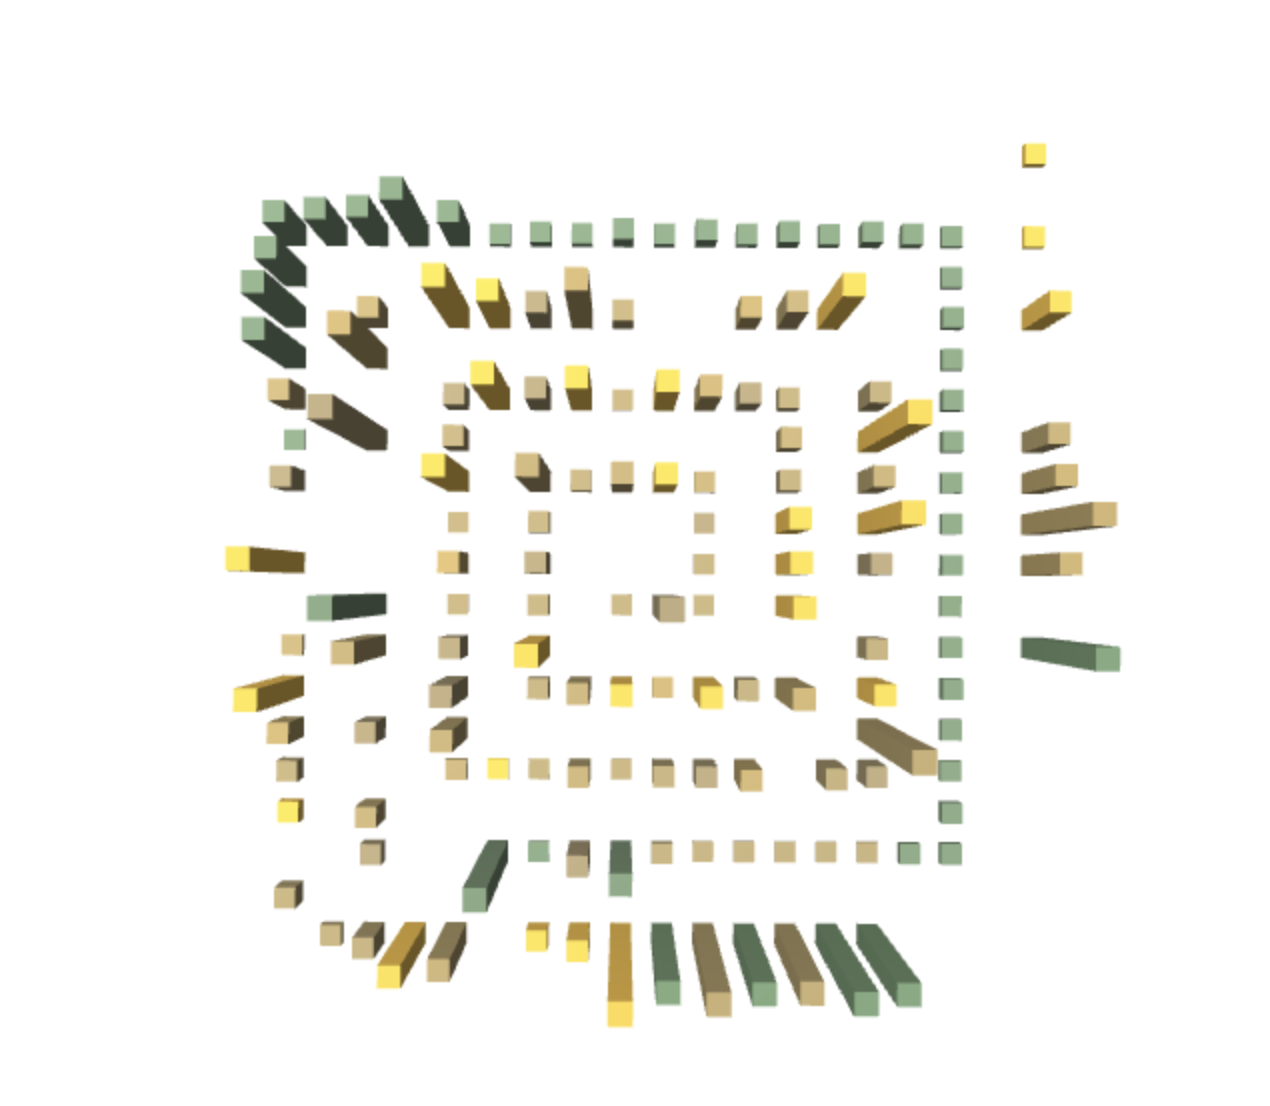
\includegraphics[width=\linewidth]{JetUML_V1S6.png}
        \caption{Month 6} \label{fig:JetUML_V1S6}
    \end{subfigure}
    
    \caption{Monthly view of JetUML} 
    \label{fig:JetUML_V1}
\end{figure}



\subsubsection*{View 2}
\textbf{Goal of this visualization}
We want to achieve the same goal as the first visualization, but this time we want to highlight our attention on Java files. 
To do that, we map Java files to entities represented by boxes and all the others to spheres with low opacity. 
To map the height of entities, we chose the SLOC metric since it is available only for Java files, so only they have a height. 

\begin{itemize}
    \item \texttt{versionGroupingStrategy}: timestamp.
    \item \texttt{versionGroupingChunkSize}: 2'629'743 (1 month). 
    \item \texttt{colorPalette}: default, additions -> green, modifications -> orange, rename -> lightblue, moves -> blue.
    \item \texttt{agingGroupingStrategy}: timestamp.
    \item \texttt{agingStepSize}: 2'629'743 (1 month).
    \item \texttt{agingSteps}: 10 steps. 
    \item \texttt{mapperStrategy}: LinearBucketValueStrategy.
    \item \texttt{mapperStrategyOptions}: max height of 20.
    \item \texttt{mapperMetricName}: SLOC. 
    \item \texttt{showUnmappedEntities}: true.
    \item \texttt{fileTypeShape}: Java -> BOX, OTHERS -> SPHERE. 
    \item \texttt{fileTypeOpacity}: Java -> BOX, OTHERS -> 0.3. 
    \item \texttt{showDeletedEntities}: false.
\end{itemize}

\textbf{Results}
Figure \ref{fig:JetUML_V2} shows the evoluition of JetUML from month 6 until the last month. 
Comparing this visualization to the previous one, Java files are much more highlighted end easy to spot. 


\begin{figure}[t!]
    \begin{subfigure}{0.48\textwidth}
    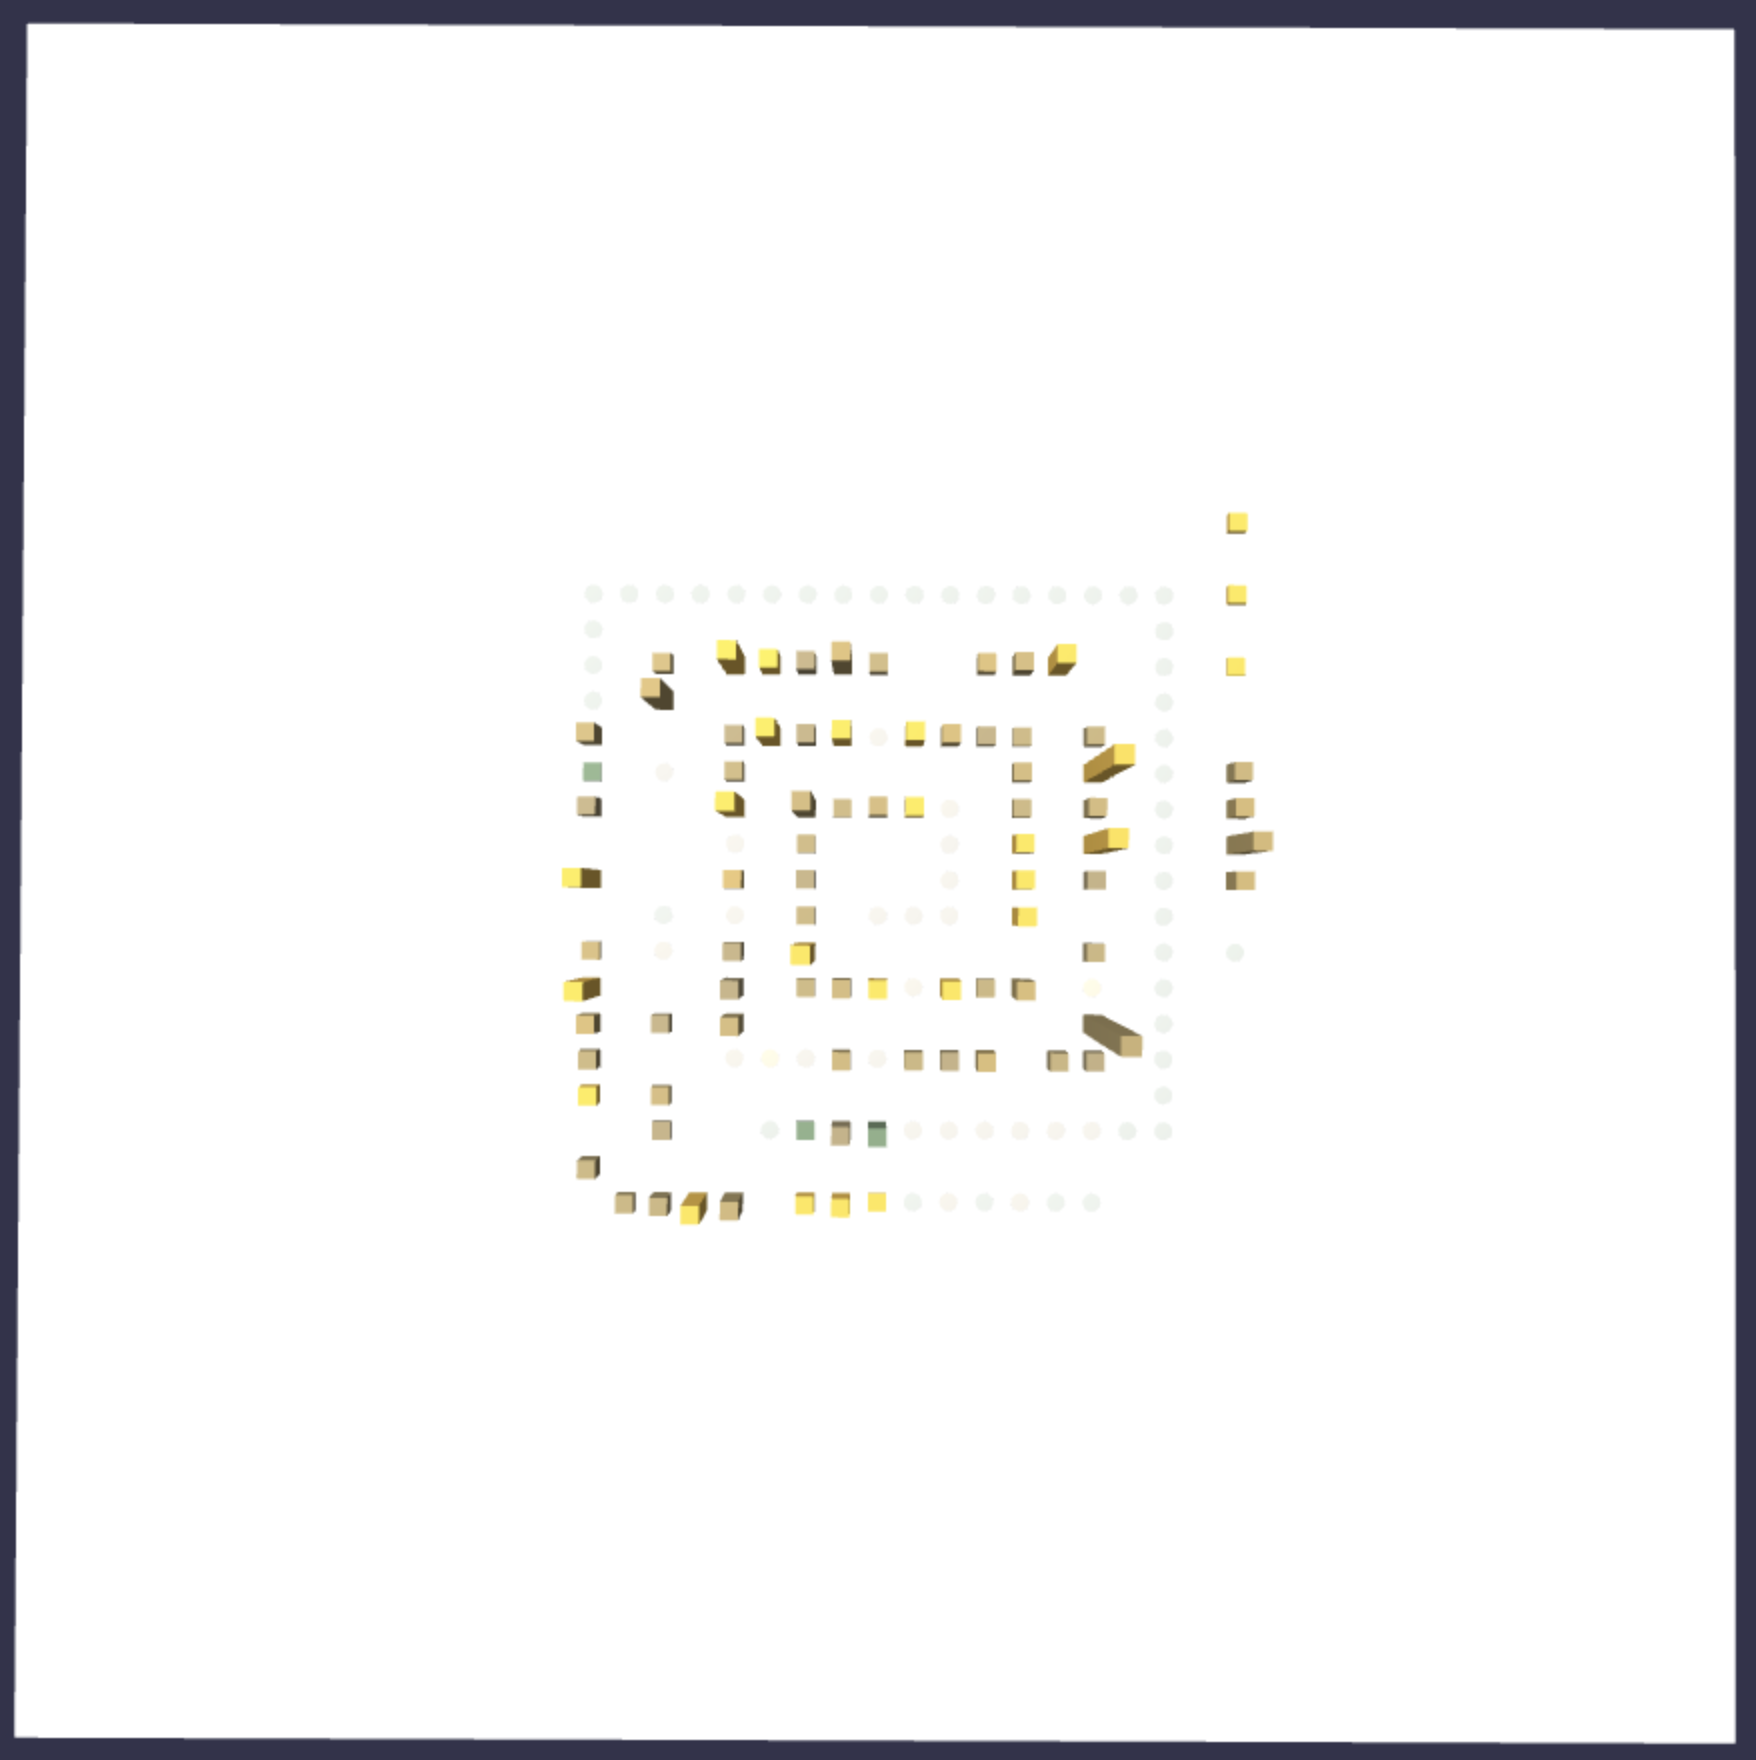
\includegraphics[width=\linewidth]{JetUML_V2S1.png}
    \caption{Month 6} \label{fig:JetUML_V2S1}
    \end{subfigure}\hspace*{\fill}
    \begin{subfigure}{0.48\textwidth}
        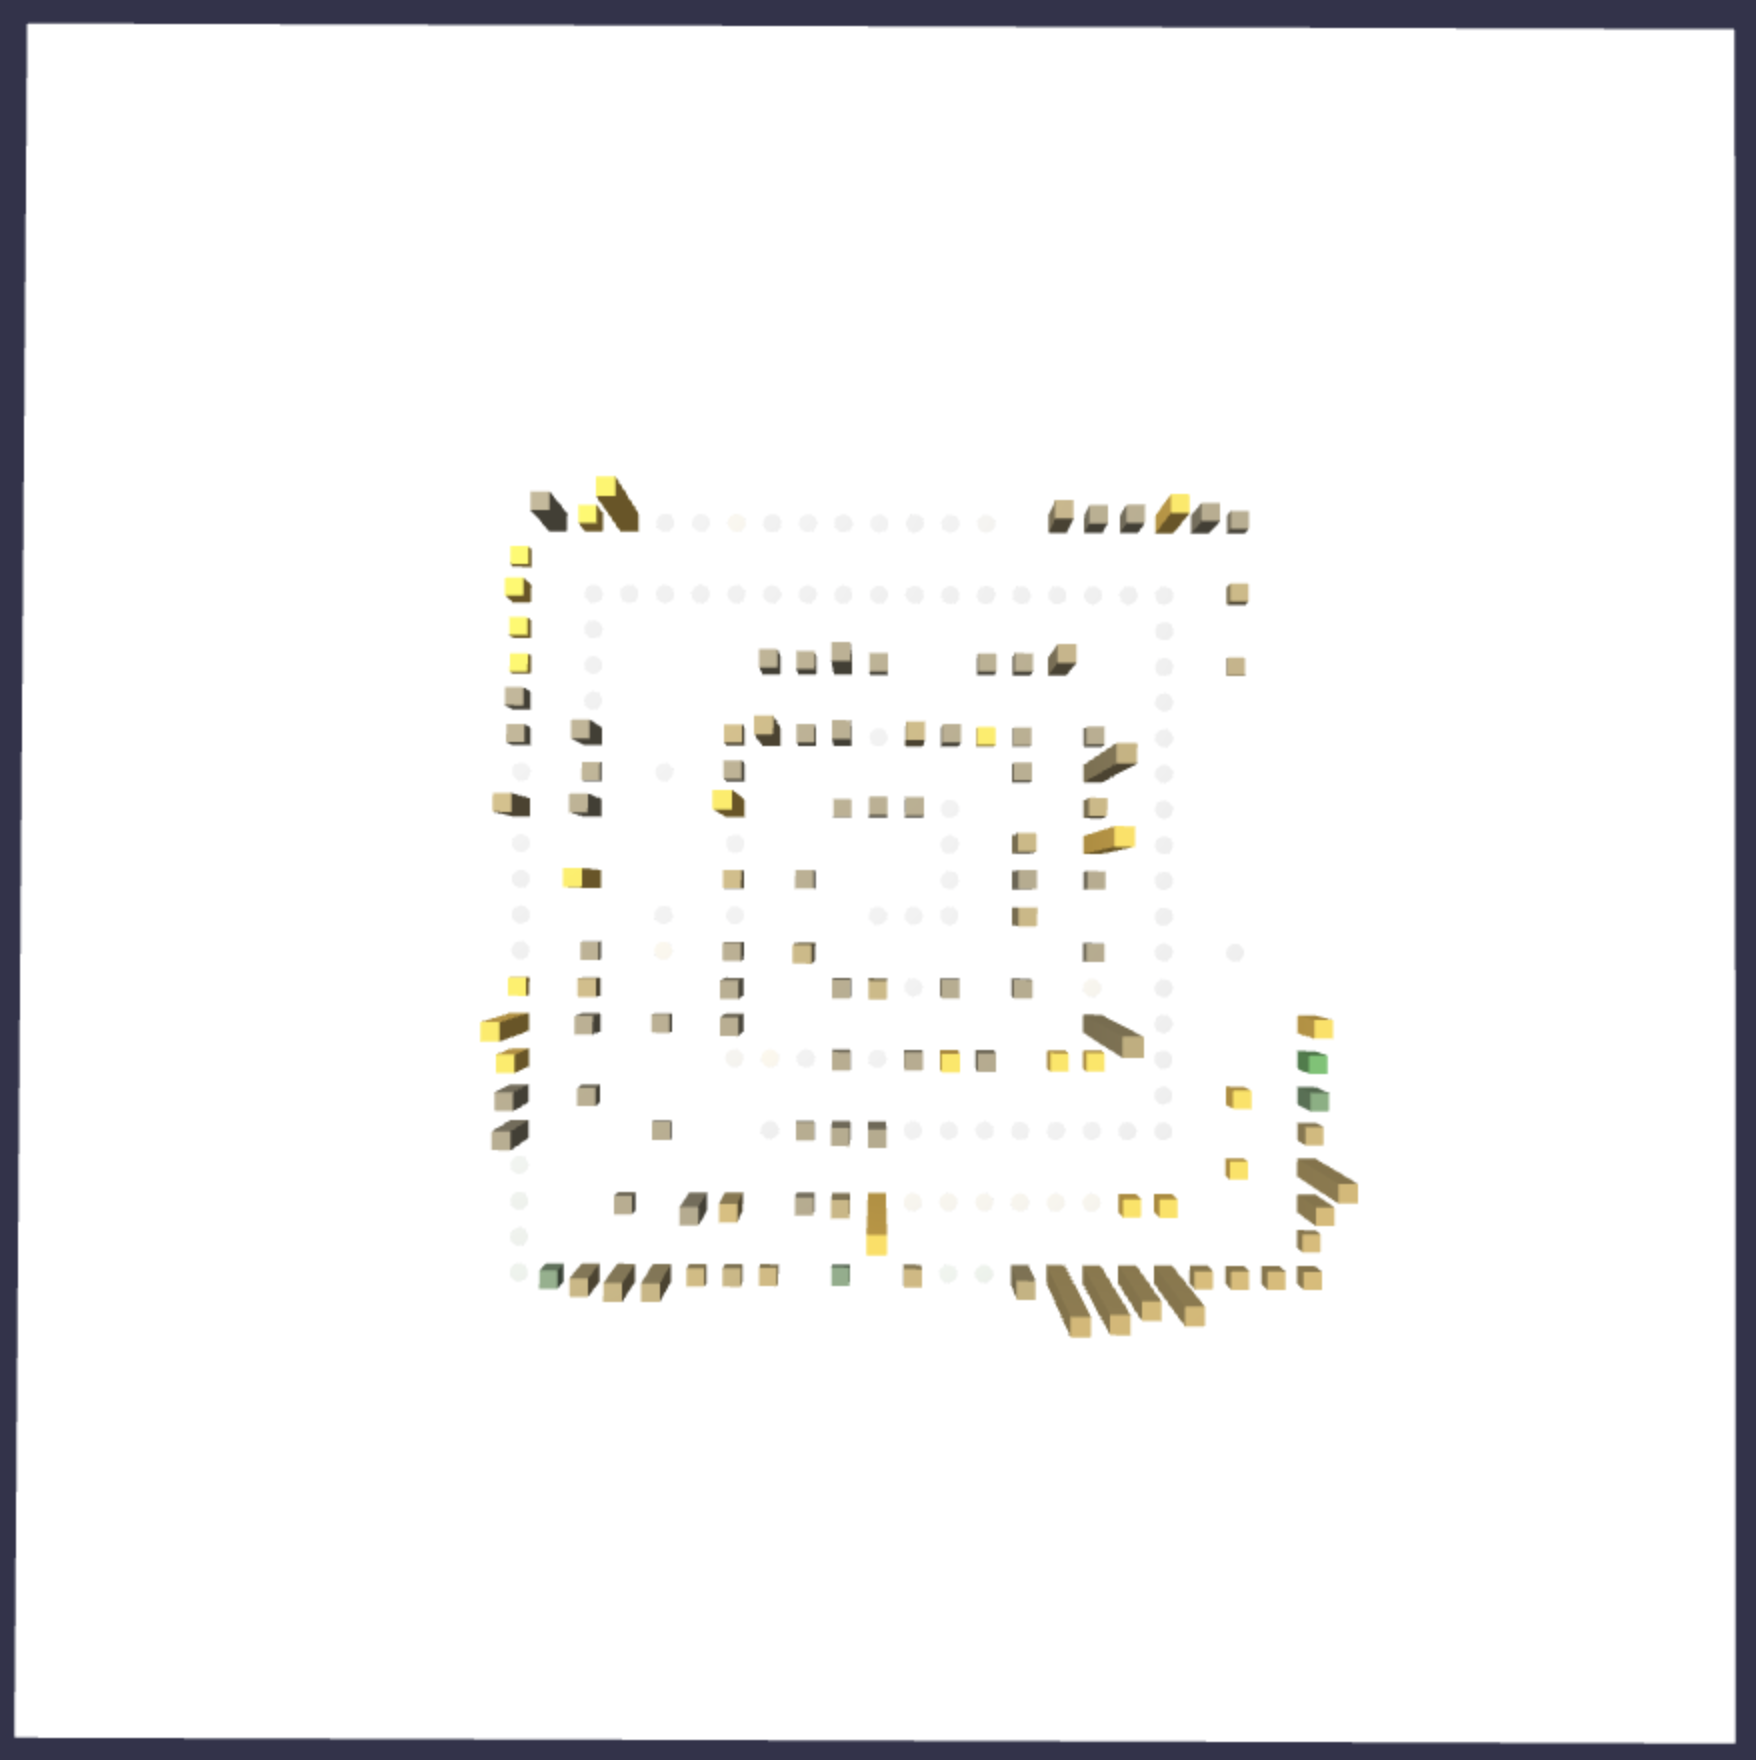
\includegraphics[width=\linewidth]{JetUML_V2S2.png}
        \caption{Month 20} \label{fig:JetUML_V2V2}
    \end{subfigure}
    
    \medskip
    \begin{subfigure}{0.48\textwidth}
        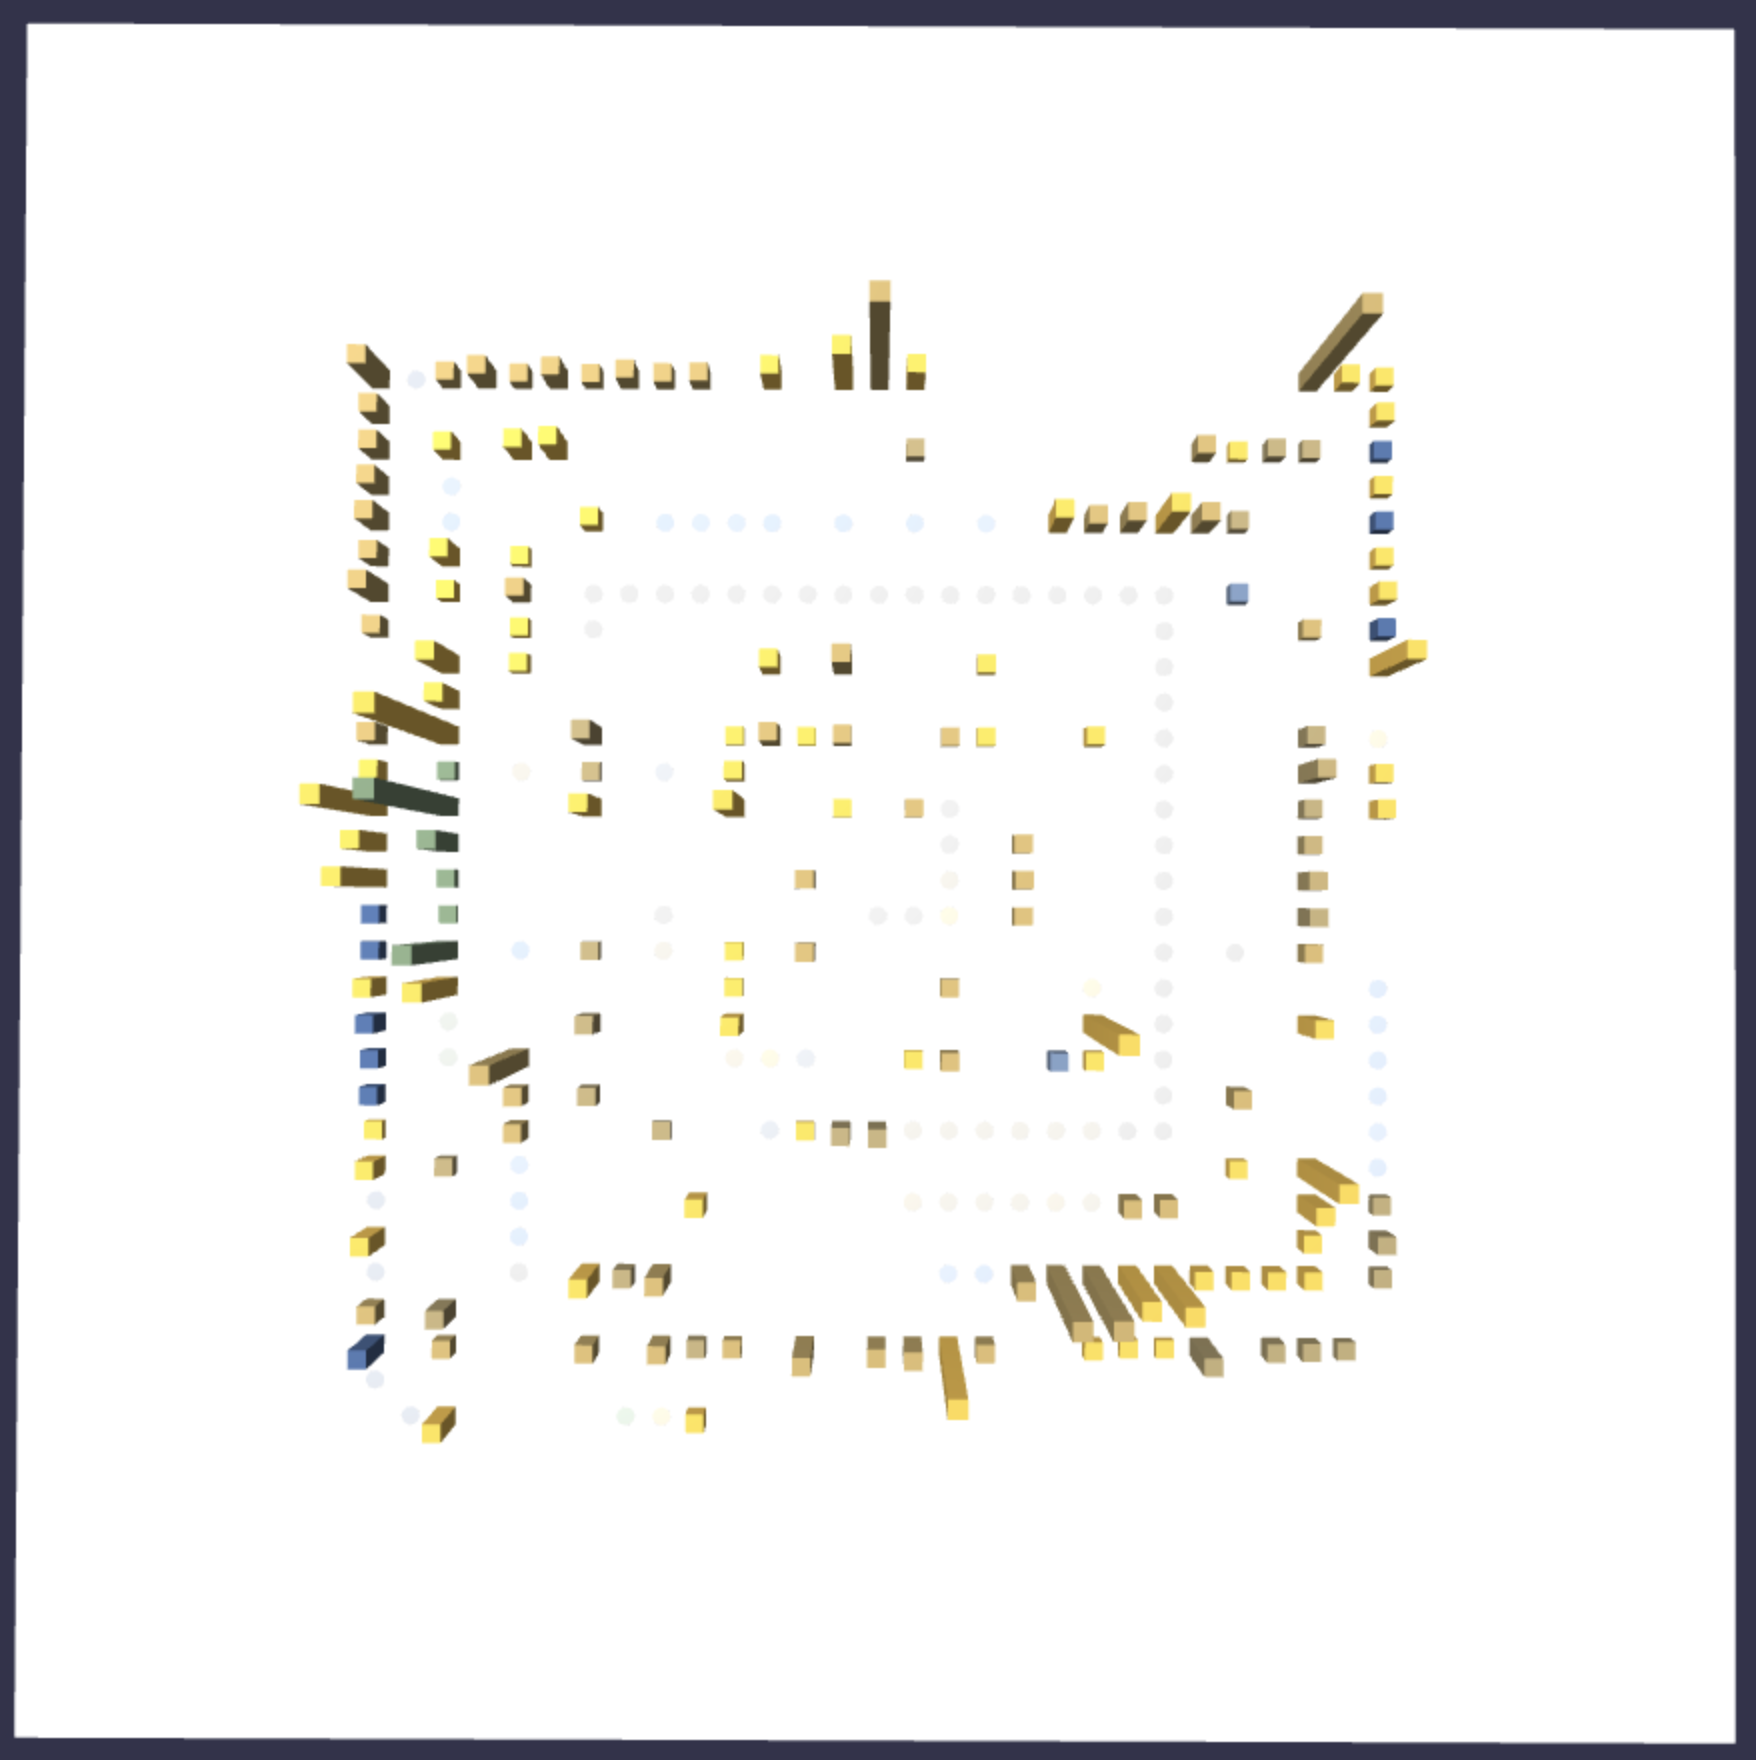
\includegraphics[width=\linewidth]{JetUML_V2S3.png}
        \caption{Month 40} \label{fig:JetUML_V2S3}
    \end{subfigure}\hspace*{\fill}
    \begin{subfigure}{0.48\textwidth}
    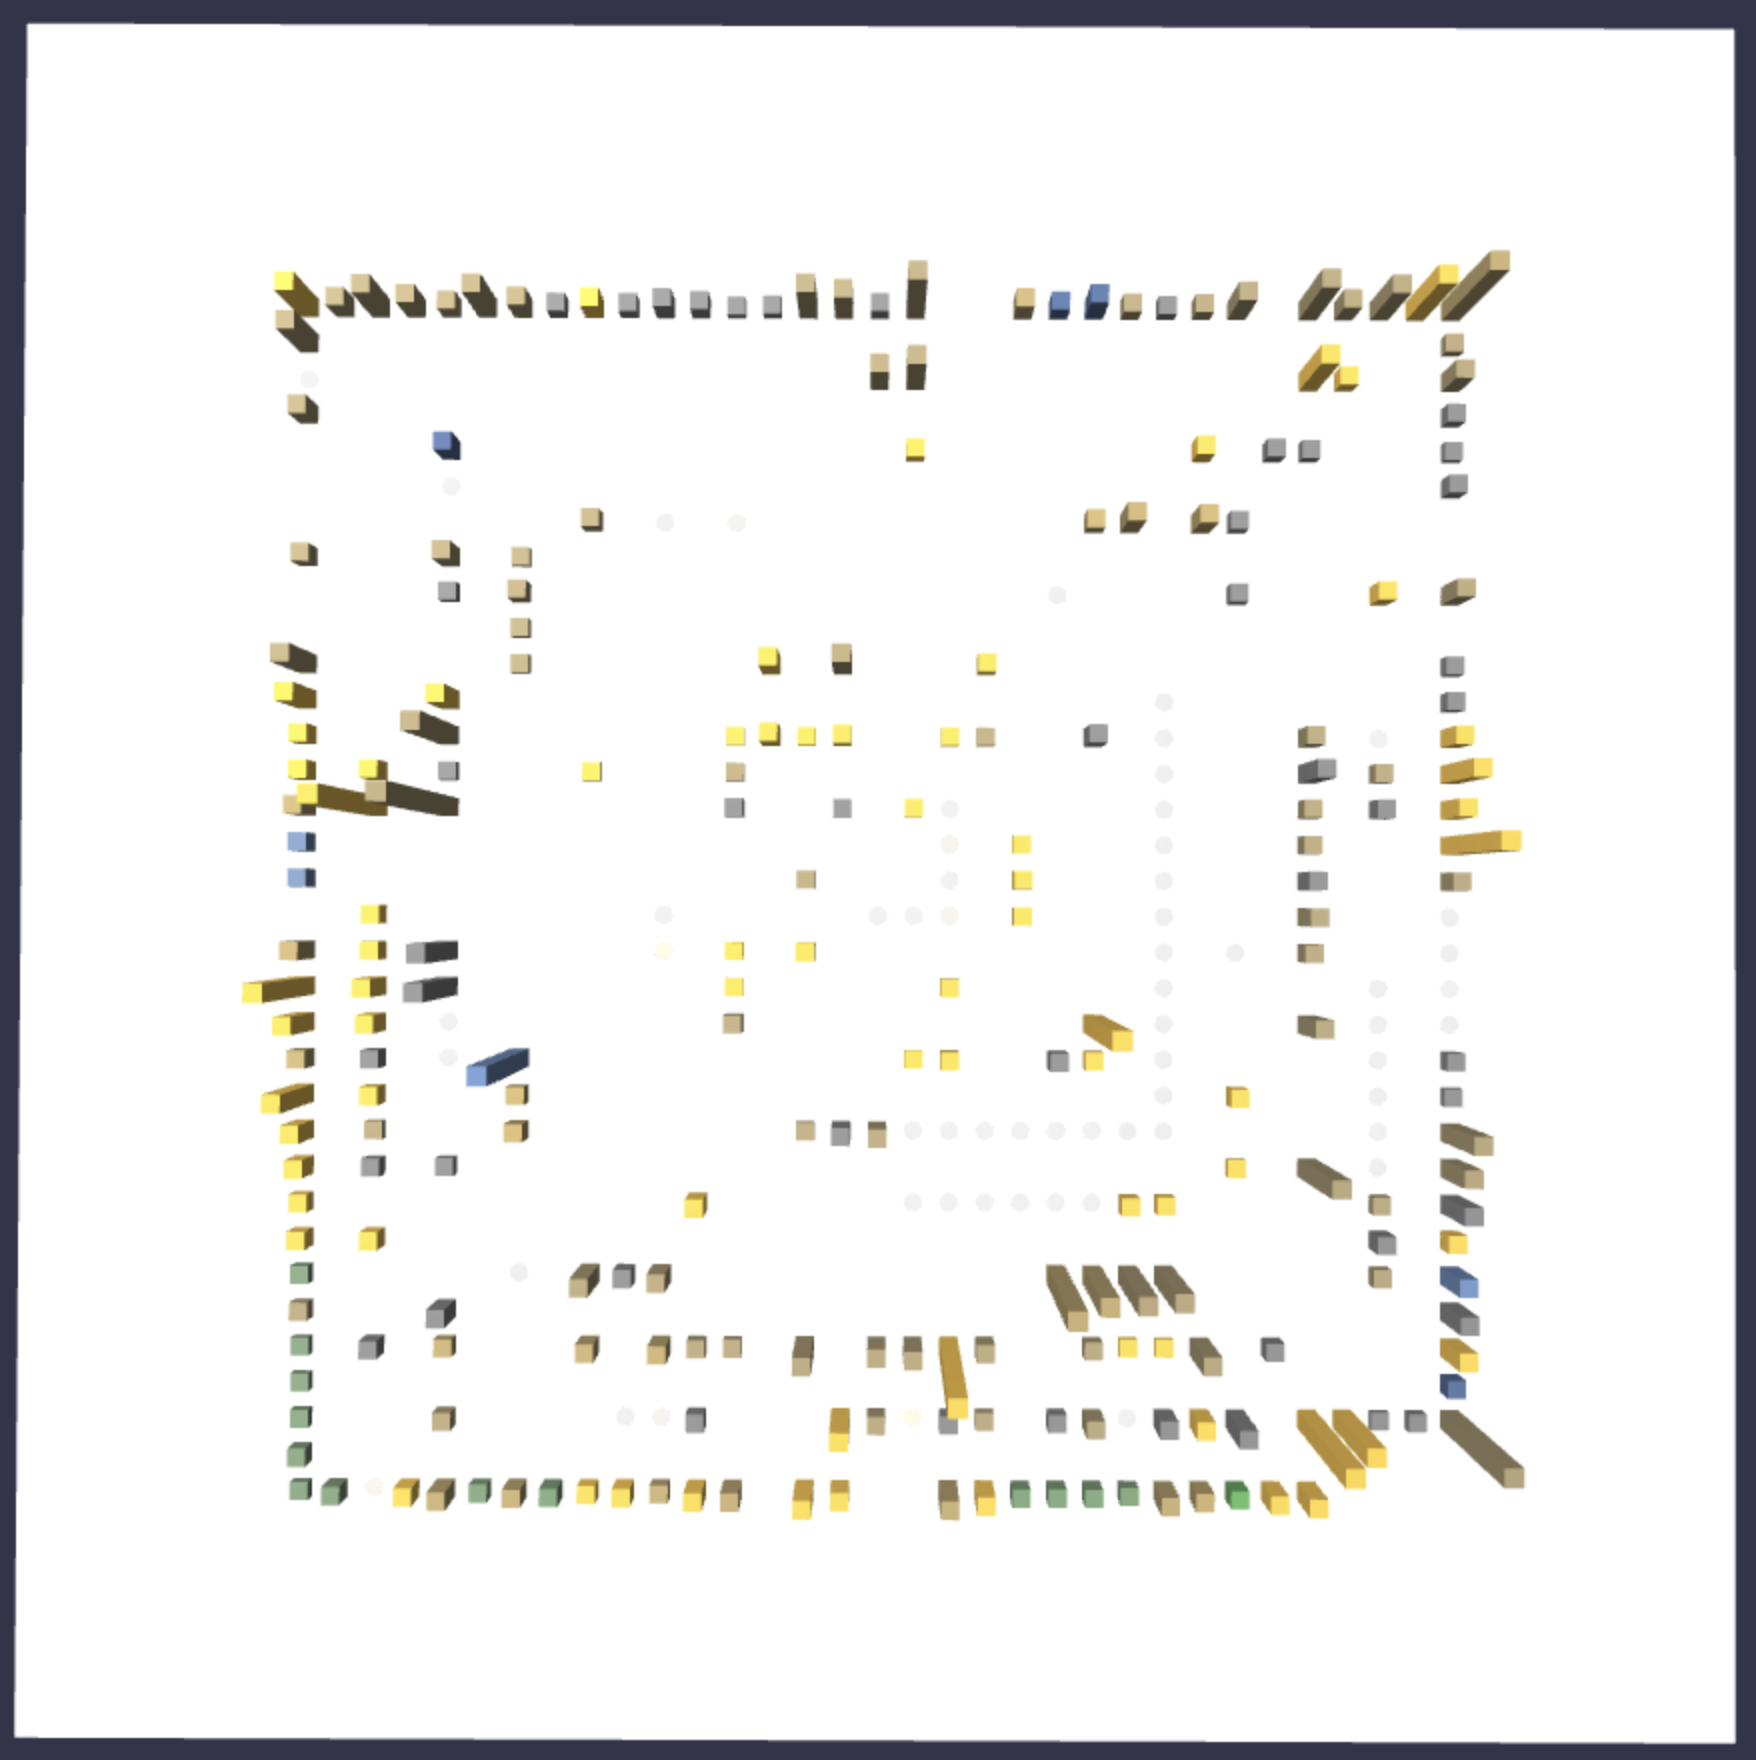
\includegraphics[width=\linewidth]{JetUML_V2S4.png}
    \caption{Month 60} \label{fig:JetUML_V2S4}
    \end{subfigure}
    
    \medskip
    \begin{subfigure}{0.48\textwidth}
        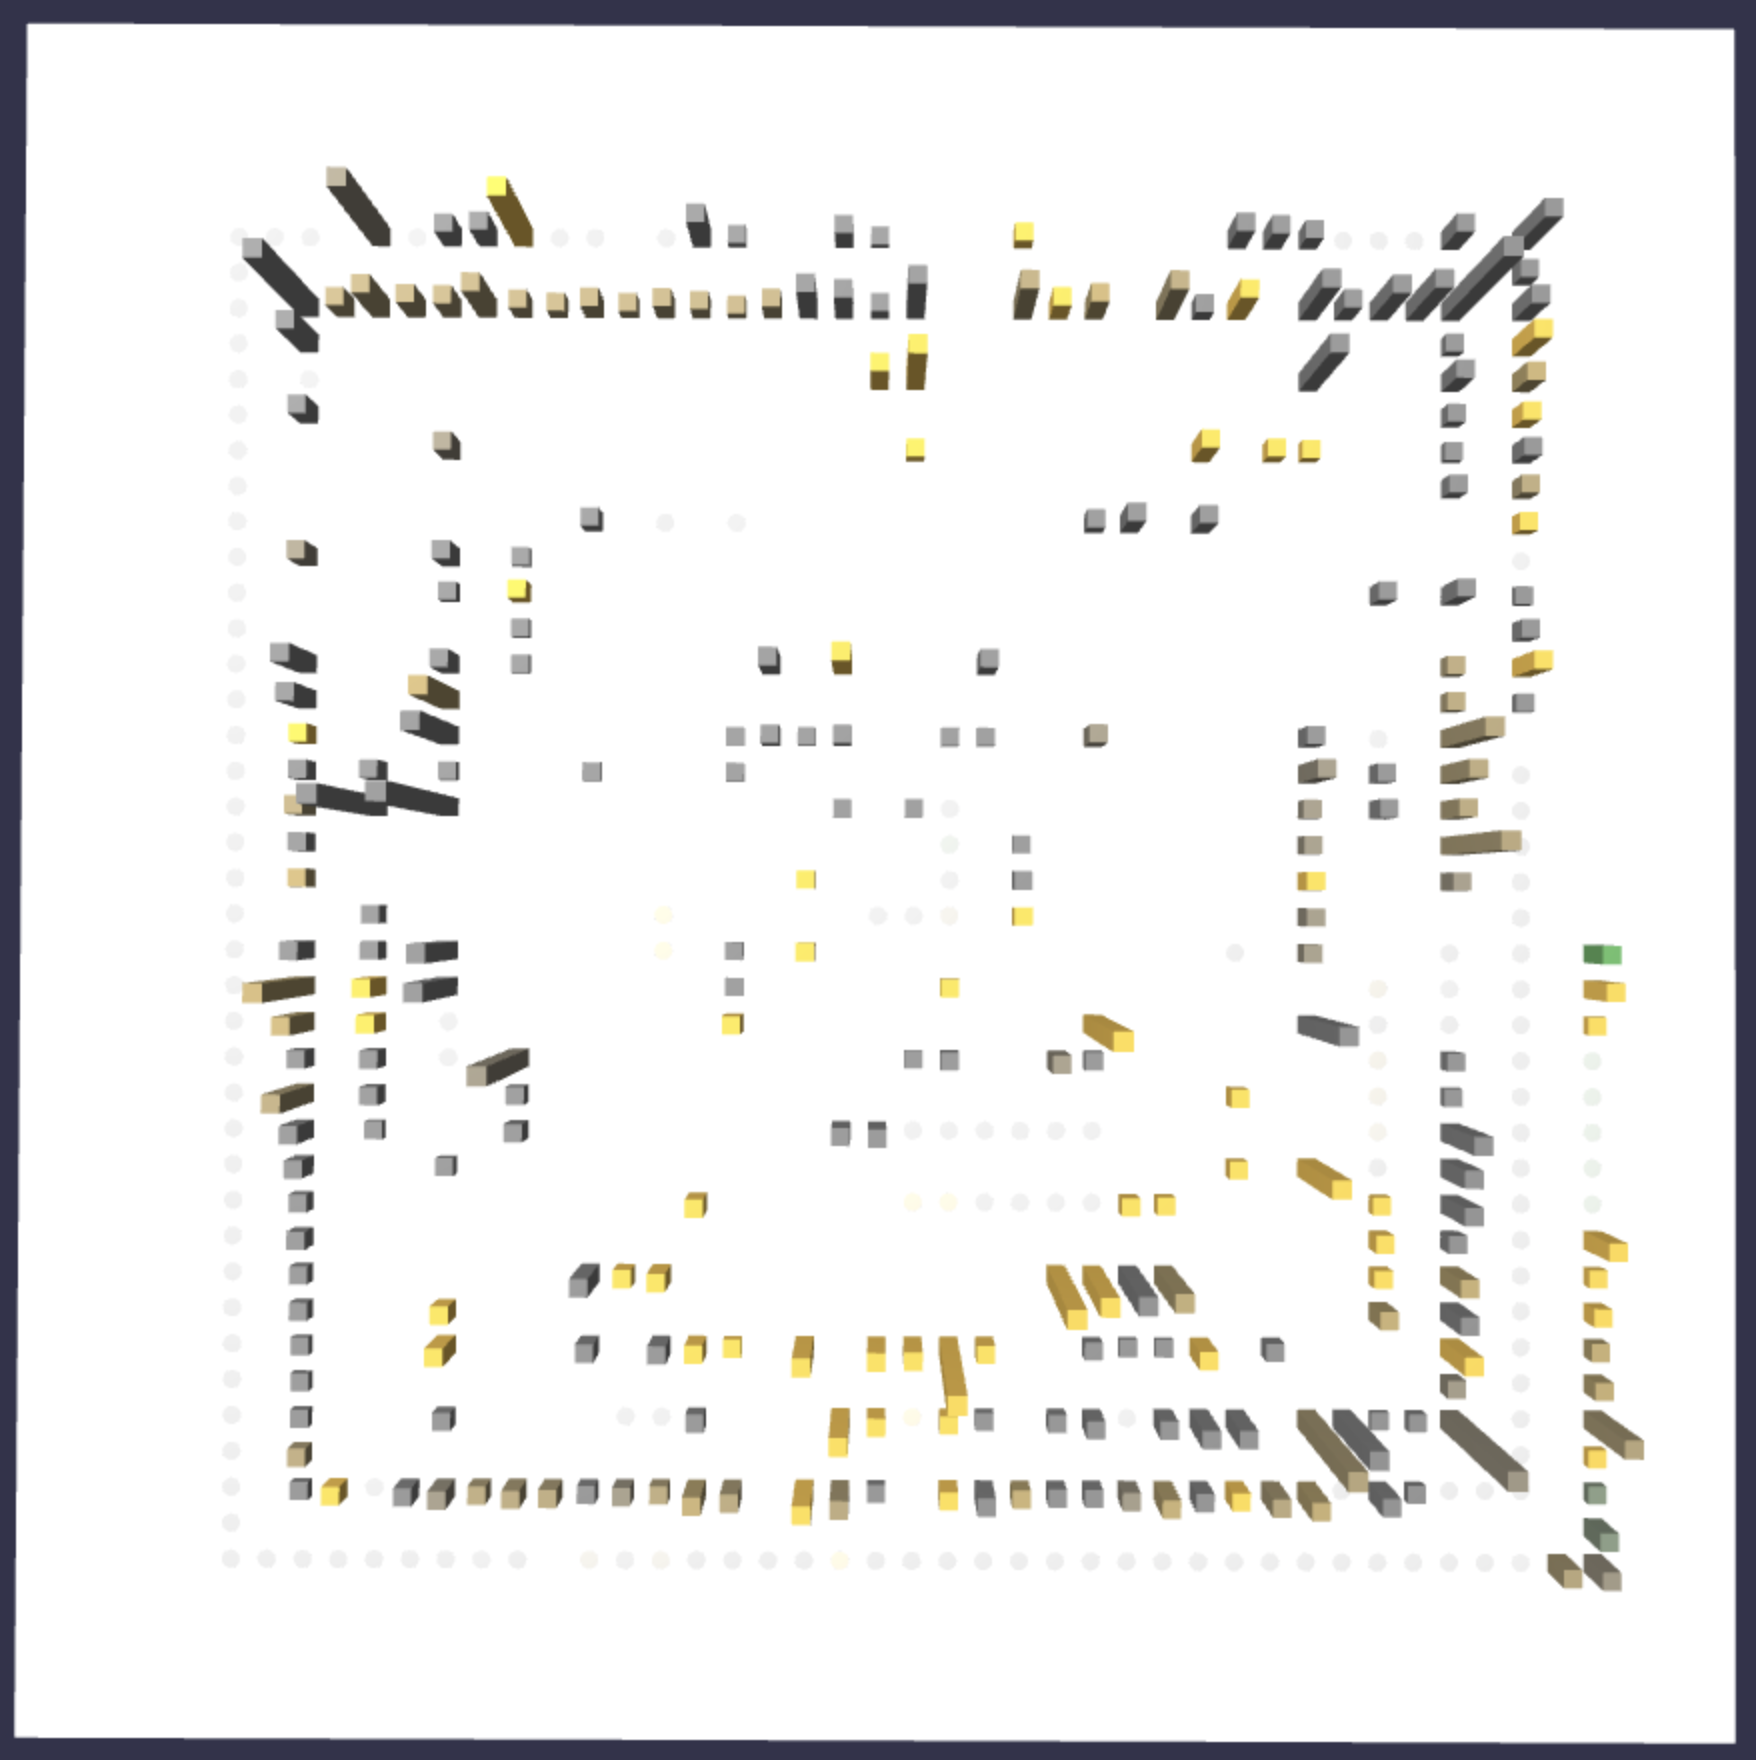
\includegraphics[width=\linewidth]{JetUML_V2S5.png}
        \caption{Month 80} \label{fig:JetUML_V2S5}
    \end{subfigure}\hspace*{\fill}
    \begin{subfigure}{0.48\textwidth}
        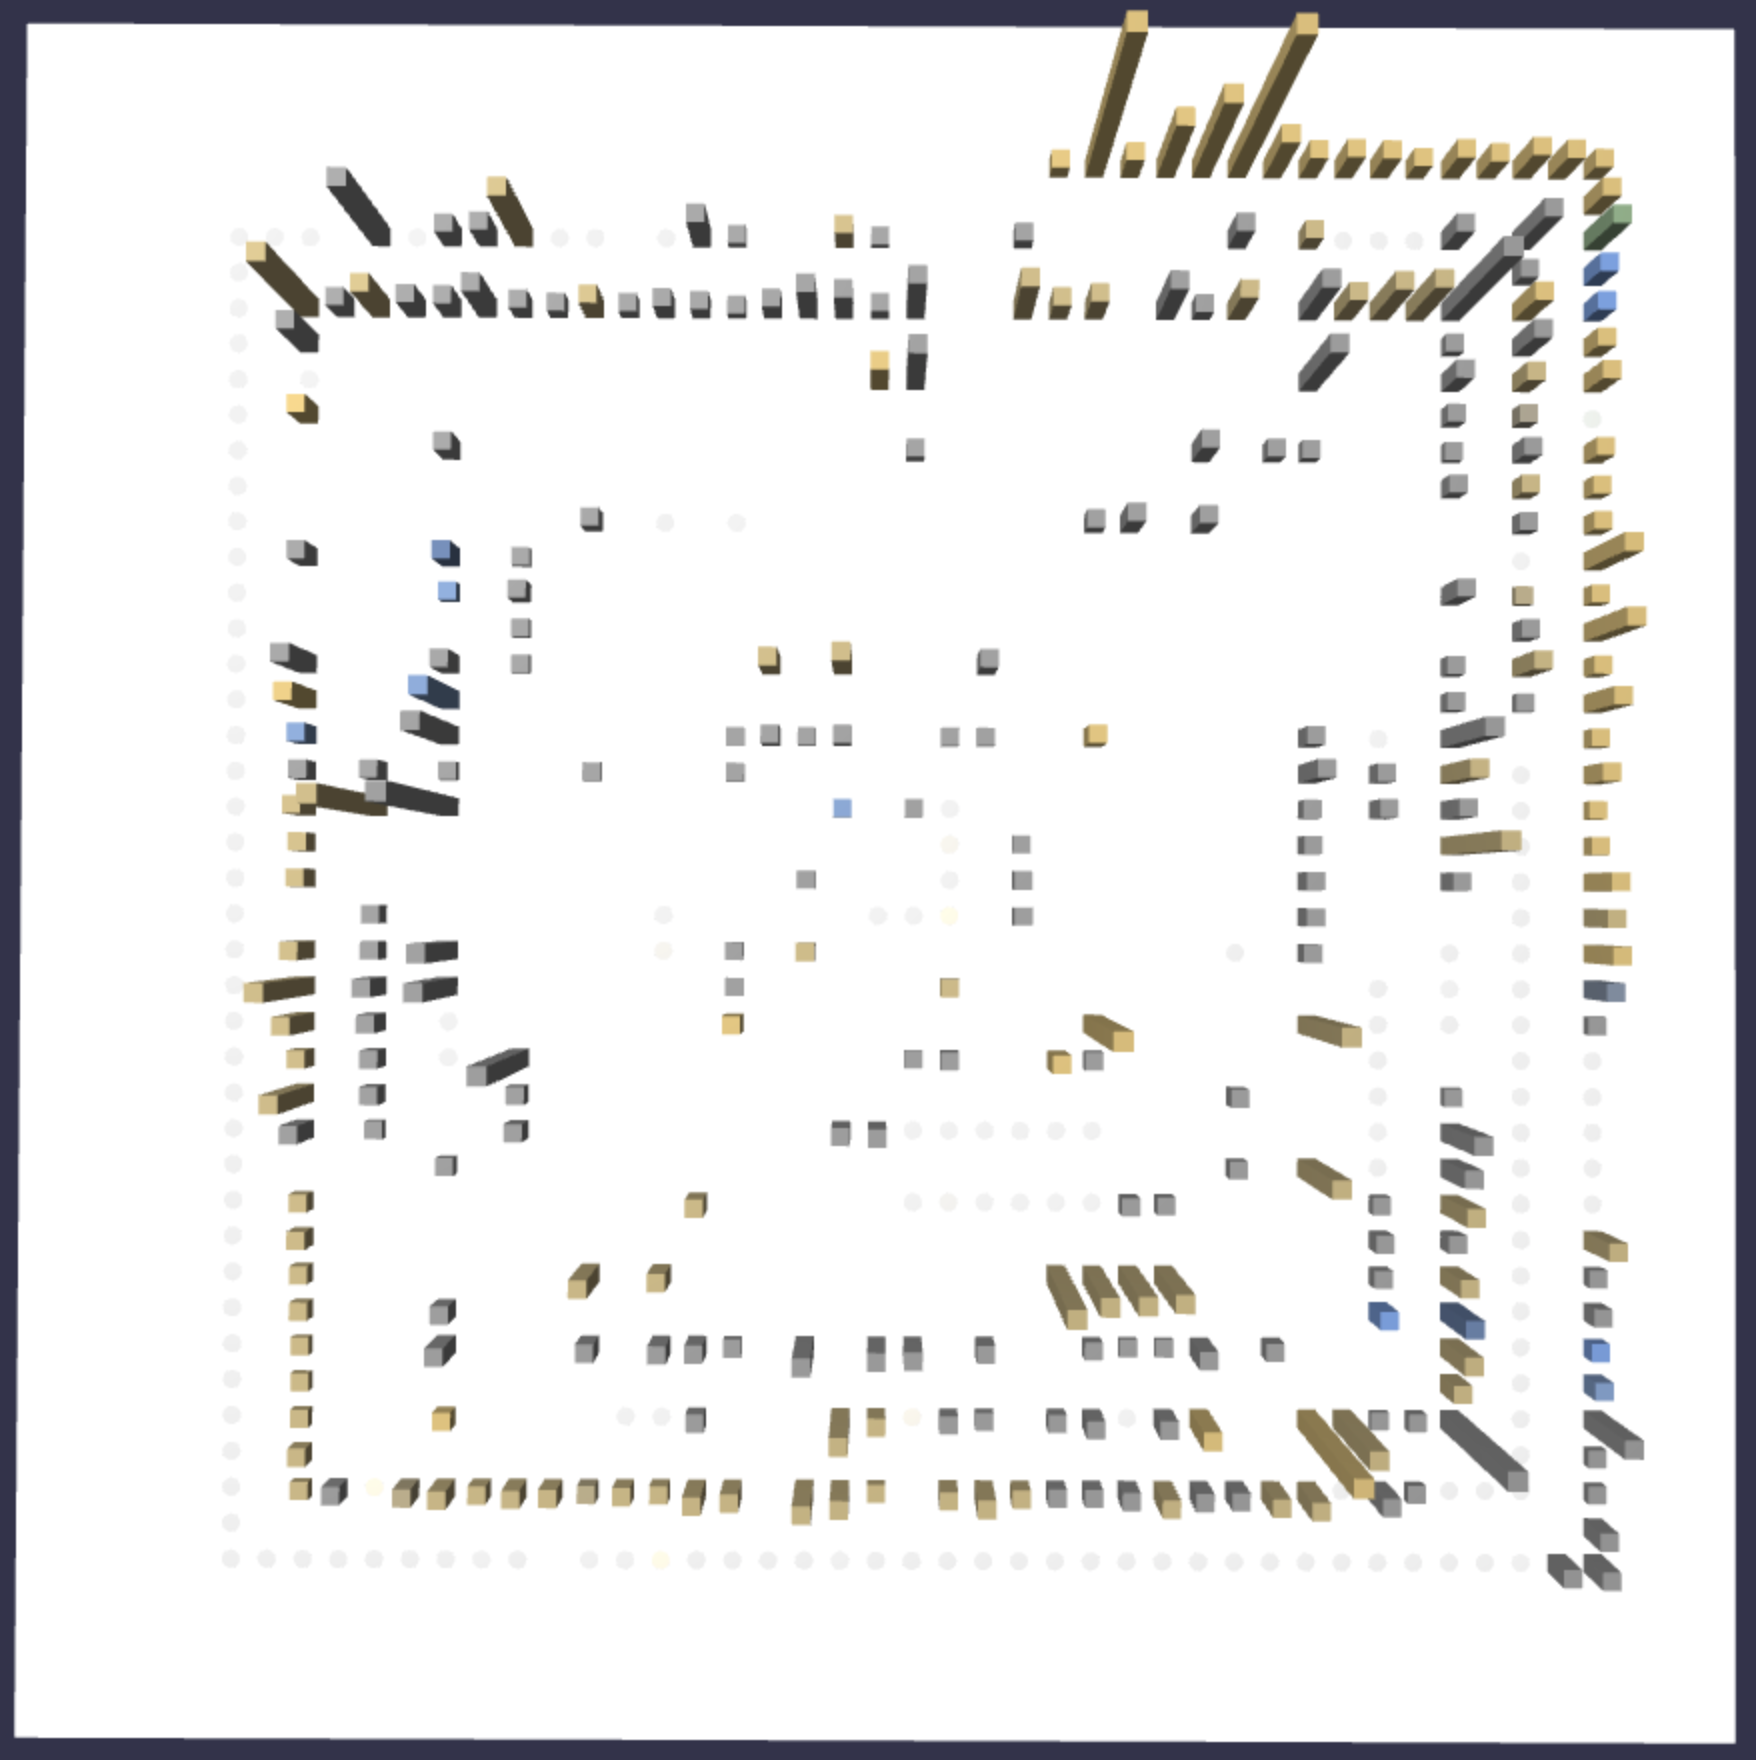
\includegraphics[width=\linewidth]{JetUML_V2S6.png}
        \caption{Month 89 (last)} \label{fig:JetUML_V2S6}
    \end{subfigure}
    
    \caption{Monthly view of JetUML} 
    \label{fig:JetUML_V2}
\end{figure}
